% Einbindung der Konfigurationsdatei
%===============================================================================
% Zentrale Layout-Angaben und Befehle
%===============================================================================
%
% F�r bessere Sicht von falschen Umbr�chen die Option draft benutzen.
% Dadurch k�nnen aber die eingebundenen Bilder nicht sichtbar sein.
\documentclass[a4paper, 12pt]{article}
%
% Hier zun�chst die ben�tigten Packages
\usepackage{german}
\usepackage[latin1]{inputenc}
\usepackage{float}
\usepackage{fancyhdr}
\usepackage[T1]{fontenc}
\usepackage{ae}
\usepackage{listings}
\usepackage{color}
\usepackage{listings}
\usepackage{bibgerm}
\usepackage{wrapfig}
\usepackage[printonlyused]{acronym}
\usepackage{url}
\usepackage{hyperref}
%
% Einbindung des Grafik-Pakets
\ifx\pdfoutput\undefined
	\usepackage[dvips]{graphicx}
\else
	\usepackage[pdftex]{graphicx}
\pdfcompresslevel=9
\pdfpageheight=297mm
\pdfpagewidth=210mm
\fi
%
% Page-Layout
\setlength\headheight{14pt}
\setlength\topmargin{-15,4mm}
\setlength\oddsidemargin{-0,4mm}
\setlength\evensidemargin{-0,4mm}
\setlength\textwidth{160mm}
\setlength\textheight{252mm}
%
% Absatzeinstellungen
\setlength\parindent{0mm}
\setlength\parskip{2ex}
%
% Kopf- und Fusszeile
\pagestyle{fancy}
\fancyhf{} % alles l�schen
\fancyhead[LO]{\footnotesize\sc\nouppercase{\leftmark}}
\fancyfoot[LO]{\footnotesize\sc Lehrstuhl f�r Praktische Informatik}
\fancyfoot[RO]{\thepage}
\renewcommand{\headrulewidth}{0pt}
\renewcommand{\footrulewidth}{0pt}
%
% Bessere Fehlermeldungen
\errorcontextlines=999
%
% Anweisung zur Erstellung der Titelseite
% #1 Bachelorarbeit || Masterarbeit
% #2 = Studiengang
% #3 = Titel der Arbeit
% #4 = Autor
% #5 = Abgabedatum
\renewcommand{\maketitle}[5]
{
\pagenumbering{Alph}
\begin{titlepage}
\centering
\begin{minipage}[t]{16cm}
\begin{minipage}{3cm}
    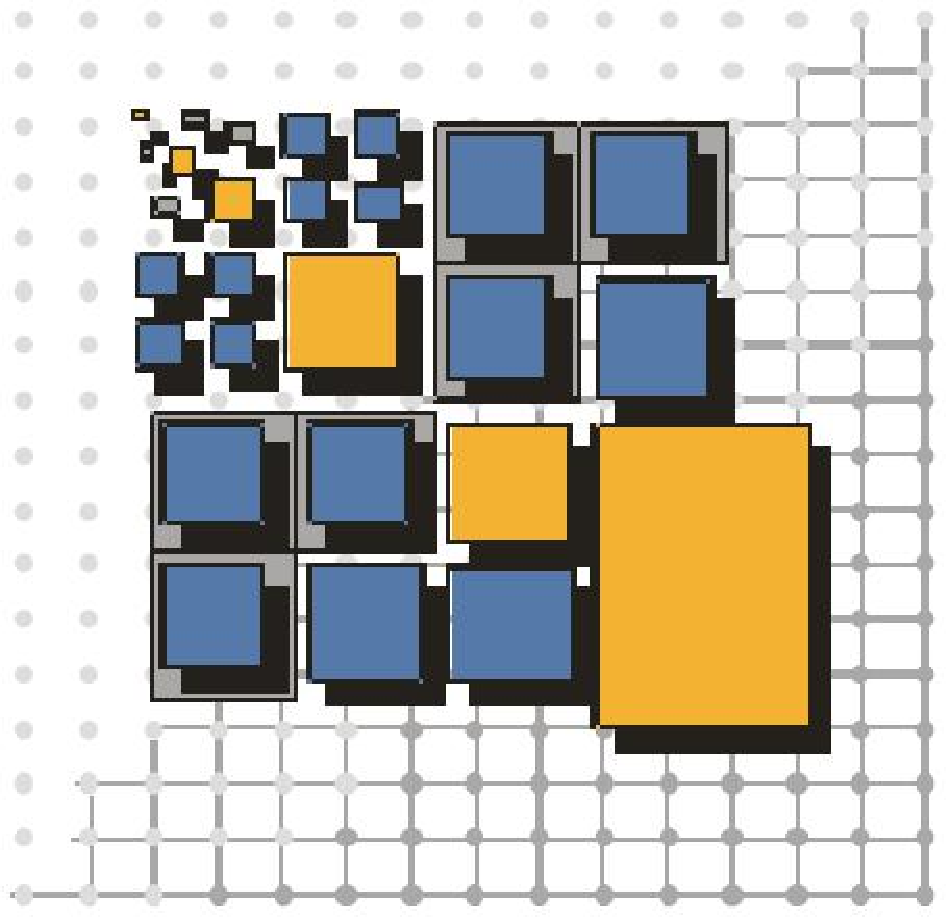
\includegraphics[height=26mm]{includes/vs-logo}
\end{minipage}
\hfill
\begin{minipage}{9cm}
  \centering
    Otto-Friedrich-Universit�t Bamberg\\[12pt]
    {\Large Lehrstuhl f�r Praktische Informatik}
\end{minipage}
\hfill
\begin{minipage}{3cm}
    
\includegraphics[height=26mm]{includes/UB-Logo-neu_blau-cmyk}
\end{minipage}
\end{minipage}\\[130pt]
{\LARGE #1}\\[24pt]
im Studiengang #2\\
der Fakult�t Wirtschaftsinformatik und Angewandte Informatik\\
der Otto-Friedrich-Universit�t Bamberg\\[90pt]
Zum Thema:\\[24pt]
{\Huge #3}\\[60pt]
\vfill
\begin{minipage}{\textwidth}
\center
Vorgelegt von:\\
{\Large #4\\[12pt]}
Themensteller:\\
Prof. Dr. Guido Wirtz\\[12pt]
Abgabedatum:\\
#5\\
\end{minipage}
\end{titlepage}
}
%
% Anweisung zur Erstellung der Eigenst�ndigkeitserkl�rung
% #1 = Typ der Arbeit
% #2 = Datum
% #3 = Vorname Name
\newcommand{\makedeclaration}[3]
{
	\fancyhead[LO]{\footnotesize\sc\nouppercase{Eigenst�ndigkeitserkl�rung}}
	%
			\vspace*{18cm}
			Ich erkl�re hiermit gem�� �17 Abs. 2 APO, dass ich die vorstehende #1 selbstst�ndig verfasst 
			und keine anderen als die angegebenen Quellen und Hilfsmittel benutzt habe.\\
			\vspace*{1cm}
			
			Bamberg, den #2 \hspace{5cm} #3
	%
}
%
% Wird f�r Hintergrund von Codelistings ben�tigt
\definecolor{hellgrau}{gray}{0.9}
%
% Einstellungen f�r Java-Code
\lstdefinestyle{javaStyle}{%
  basicstyle=\small,%
  backgroundcolor=\color{hellgrau},%
  keywordstyle=\bfseries,%
  showstringspaces=false,%
  language=Java,%
  numbers=left,%
  numberstyle=\tiny,%
  stepnumber=1,%
  numbersep=5pt,%
  extendedchars=true,%
  xleftmargin=2em,%
  lineskip=-1pt,%
  breaklines%
}
%
% neues environment f�r Java-Sourcecode
% #1 = "caption={Hier eigene �berschrift}, label={Hier eigenes Label}"
\lstnewenvironment{javacode}[1][]{%
\lstset{style=javaStyle,#1}%
}{}
%
% Befehl zum Einbinden von Java-Sourcecode aus Datei
% #1 = Dateiname relativ zu src-Verzeichnis
% #2 = �berschrift
% #3 = Label
\newcommand{\javafile}[3]{%
   \lstinputlisting[%
     caption={#2},%
     label={#3},%
     style=javaStyle]{src/#1}%
}
%
% Einbindung eines Bildes
% #1 = label f�r \ref-Verweise
% #2 = Name des Bildes ohne Endung relativ zu images-Verzeichnis
% #3 = Beschriftung
% #4 = Breite des Bildes im Dokument in cm
\newcommand{\bild}[4]{%
  \begin{figure}[htb]%
    \begin{center}%
      \includegraphics[width=#4cm]{images/#2}%
      \vskip -0.3cm%
      \caption{#3}%
      \vskip -0,2cm%
      \label{#1}%
    \end{center}%
  \end{figure}%
}
%
% Umgebung f�r Fliesstext um Grafik
% #1 = Ausrichtung: r, l, i, ...
% #2 = Breite des Bildes in cm
% #3 = Name des Bildes ohne Endung relativ zu images-Verzeichnis
% #4 = Beschriftung
% #5 = label f�r \ref-Verweise
\newcommand{\fliesstext}[5]{%
\begin{wrapfigure}{#1}{#2cm}%
\includegraphics[width=#2cm]{images/#3}%
\caption{#4}%
\label{#5}%
\end{wrapfigure}%
}
%%% Local Variables:
%%% mode: latex
%%% TeX-master: t
%%% End:


\begin{document}

% Titelblatt erstellen
\maketitle{Bachelorarbeit}{Wirtschaftsinformatik}{Automatisierung der Datenerfassung f�r Wissensdatenbanken im technischen Kontext}{Petr Vasilyev}{16.05.2017}

% Erstellung der Inhaltsverzeichnisses
\pagenumbering{Roman}

\tableofcontents
\newpage

\listoffigures
\newpage

\listoftables
\newpage

\lstlistoflistings
\newpage

\fancyhead[LO]{\footnotesize\sc\nouppercase{Abk�rzungsverzeichnis}}
\section*{Abk�rzungsverzeichnis}
% In Klammern steht das l�ngste Akronym!
\begin{acronym}[MVVM]
 \acro{API}{Application Programming Interface}
 \acro{DOM}{Document Object Model}
 \acro{DSS}{Decision Support System}
 \acro{DTD}{Document Type Definition}
 \acro{HTML}{Hypertext Markup Language}
 \acro{HTTP}{Hypertext Transfer Protocol}
 \acro{JSON}{JavaScript Object Notation}
 \acro{MVVM}{Model View ViewModel}
 \acro{PaaS}{Platform-as-a-Service}
 \acro{REST}{Representational State Transfer}
 \acro{SHA}{Secure Hash Algorithm}
 \acro{URI}{Uniform Resource Identifier}
 \acro{URL}{Uniform Resource Locator}
 \acro{XML}{Extensible Markup Language}
 \acro{XPath}{XML Path Language}
\end{acronym}
\newpage
\fancyhead[LO]{\footnotesize\sc\nouppercase{\leftmark}}
\setcounter{page}{1}
\pagenumbering{arabic}

%
% Einzelne Kapitel mit \input{sections/Kapitel-File} einf�gen.
%
\section{Einf�hrung}\label{sec:Einf�hrung}
\subsection{Motivation}\label{subsec:Motivation}
Die Idee von wissensbasierten Systemen entstand aus dem Anliegen, ein intelligentes System zu schaffen, das mittels spezifischen Wissens die Fachexperten bei den Probleml�sungen unterst�tzt \cite[S.18]{akerkar2010}. Darin besteht der Unterschied zwischen einem konventionellen Informationssystem und einem wissensbasierten System. Informationssysteme sind datenbasiert aufgebaut und konzentrieren sich auf Datenverarbeitung \cite[S.19]{akerkar2010}. Eine Spezialisierung der wissensbasierten Systeme stellen Expertensysteme dar, in denen das Wissen letztendlich von Experten stammt. Ein wissensbasiertes System bzw. ein Expertensystem ist durch die Trennung zwischen der Wissensdarstellung eines Problembereichs und der Wissensverarbeitung gekennzeichnet \cite[S.11]{beierle2014}.\\ 
Die Beschreibung des Wissens von einem wissensbasierten bzw. Expertensystem erfolgt in der Wissensbasis, die in Form einer Wissensdatenbank realisiert wird. Die Anfangswissensbasis wird in der Regel mithilfe manueller Datenerfassung aufgebaut \cite[S.70]{kurbel1992}. Ein Interview zwischen einem Wissensingenieur und einem Wissenstr�ger wird beispielsweise oft eingesetzt \cite[S.76]{gottlob1990}. Allerdings sind die manuellen Wissenserwerbsmethoden f�r die Weiterentwicklung der Wissensbasis hinsichtlich der Erweiterung und Aktualisierung der Wissensdatenbank eher schlecht geeignet, da sie fehleranf�llig, kosten- und zeitintensiv sind. Aus diesem Grund gibt es Bestrebungen, den Prozess der Datenerfassung zu automatisieren. Eine Auswahl an bestehenden Ans�tzen, die bez�glich der vorliegenden Arbeit relevant sind, wird im Abschnitt zu den verwandten Arbeiten gegeben. Trotz der vielen Herangehensweisen gibt es kein einheitliches Konzept, das einen allgemeinen Rahmen f�r die Automatisierung der Datenerfassung bildet.
\subsection{Zielsetzung}\label{subsec:Zielsetzung}
Das Ziel der vorliegenden Arbeit ist die Erarbeitung eines allgemeinen Konzeptes zur Automatisierung der Datenerfassung. Da die komplett automatisierte Datenerfassung sehr schwierig umzusetzen ist, liegt der Schwerpunkt dieser Arbeit auf der Kombination zwischen den manuellen und maschinellen Vorgehensweisen.\\
Beim technischen Kontext wird angedeutet, dass die Umsetzung im Rahmen eines bestimmten Anwendungsbereichs erfolgt. Es wird also kein Allgemeinwissen wie in \cite{tandon2016}, sondern ein anwendungsbezogenes Wissen betrachtet. In diesem Zusammenhang wird das Konzept auf Basis eines Expertensystems entwickelt, da die Wissensbasis eines Expertensystems spezifischer ist als bei einem wissensbasierten System.\\
Die praktische Umsetzung soll auf Basis von \textit{PaaSfinder}\footnote{https://paasfinder.org} erfolgen. Bei \textit{PaaSfinder} handelt es sich um eine Web-Anwendung, die �ber eine Wissensdatenbank im Bereich \ac{PaaS} verf�gt. \ac{PaaS} geh�rt neben \ac{IaaS} und \ac{SaaS} zum Themengebiet von Cloud Computing \cite{nist2011} und soll die Anwendungsentwicklung erleichtern, indem die Laufzeit- ober Entwicklungsumgebungen von einem \ac{PaaS}-Anbieter dem Kunden vorkonfiguriert angeboten werden \cite[S.14]{lawton2008}. Da \textit{PaaSfinder} ein Open-Source Projekt ist, kann jeder der Datenbank von \textit{PaaSfinder} beitragen. Allerdings ist die Mitwirkung mit einem hohen Aufwand verbunden und setzt Informatikkenntnisse voraus. Au�erdem werden die Daten von \textit{PaaSfinder} haupts�chlich auf den Webseiten von \ac{PaaS}-Anbietern manuell erfasst. Dies stellt ein hohes Entwicklungspotential, die Erfassung von solchen Daten zu automatisieren.
\subsection{Verwandte Arbeiten}\label{subsec:Verwandte-Arbeiten}
Der Ausgangspunkt dieser Arbeit stellt die Publikation \cite{tecuci1992} von G. Tecuci dar, die die Automatisierung der Wissenserfassung als ein Konzept der Erweiterung, Aktualisierung und Verbesserung der Wissensbasis beschreibt \cite[S.1444]{tecuci1992}. In diesem Zusammenhang wurde ein lernendes System vorgestellt, das eine Auswahl an generischen Ans�tzen des maschinellen Lernens bei der Wissenserfassung umsetzt \cite[S.1445]{tecuci1992}. Ferner wird ein Framework gebildet, das die Wissenserfassung durch maschinelles Lernen automatisiert. Dar�ber hinaus werden die gelernten Daten von einem Experten auf die Korrektheit �berpr�ft. Die Entwicklung der Wissensbasis wird in drei Phasen durchgef�hrt. In der ersten Phase wird die Anfangswissensbasis aufgebaut, die unvollst�ndig und teilweise widerspr�chlich sein kann. Die zweite Phase umfasst die inkrementelle Erweiterung und Verbesserung der Wissensbasis. Schlie�lich wird in der dritten Phase die Wissensbasis in Bezug auf Effizienz optimiert \cite[S.1444]{tecuci1992}. Die Kernaussage der Arbeit besteht darin, dass die Kooperation zwischen dem fachlichen Experten und dem Expertensystem in jeder Phase die Automatisierung der Datenerfassung deutlich erleichert. Beispielsweise k�nnen die Daten von einem Algorithmus generiert werden. Daraufforgend werden sie vom fachlichen Experten auf die formale und semantische Korrekteit �berpr�ft und in die Wissensbasis gespeichert \cite[S.1445]{tecuci1992}. In \cite{tecuci1994} wird die Entwicklung des Frameworks fortgef�hrt, wobei der Schwerpunkt im Bereich vom multi-strategischen Lernen (multistrategy leraning) liegt \cite[S.137]{tecuci1994}.\\
Neben \cite{tecuci1992} und \cite{tecuci1994} gibt es eine Reihe weiterer Ans�tze, die das maschinelle Lernen bei der Automatisierung der Datenerfassung zur Hifle nehmen. Einige Beispiele sind \cite{castro1999}, \cite{castro2001}, \cite{webb1996}. Dabei ist die Idee der Zusammenarbeit zwischen dem Experten und dem Lernalgorithmus durchaus verbreitet. Ein Beispiel stellt die Arbeit von Castro et al. \cite{castro2001} dar. In der grundlegenden Idee beziehen sich die Autoren auf die Arbeit von \cite{tecuci1992}. Als Startpunkt wird eine unvollst�ndige Anfangswissensbasis betrachtet, die schrittweise verbessert wird, indem der Experte die Fragen vom System beantwortet. Bei der Frageerstellung wird ein Lernalgorithmus eingesetzt, der aus einer Trainingsmenge die Regeln lernt und kontinuierlich die Qualit�t der Fragen verbessert. Dabei betonen Castro et al. \cite{castro2001}, dass der Lernalgorithmus keineswegs den Wissensingenieur ersetzen kann. Vielmehr soll der Algorithmus den Wissensingenieur die Routinearbeit abnehmen und bei den schwierigeren Aufgaben unterst�tzen, indem verschiedene Varianten der Interviews vom Algorithmus vorgeschlagen werden \cite[S.308]{castro2001}.\\
Ein praxisorientierter Ansatz f�r die Autormatisierung der Wissenserfassung wird in \cite{gebus2009} thematisiert. Allgemein handelt es sich um die Transformation eines datenbasierten Systems in ein wissensbasiertes System, um die Effizient der Produktion zu steigern. Im Hinblick auf die Automatisierung der Aktualisierung und Erweiterung der unvollst�ndigen Wissensbasis beziehen sich Gebus und Leivisk{\"a} auf die Erkenntnisse aus \cite{tecuci1992}, \cite{winter1992} und \cite{su2002}. Bez�glich der Erfassung von Erfahrungswissen nehmen die Autoren den Bezug auf die Arbeit von Okamura et al \cite{okamura1991}, die Heuristik bei Probleml�sungen eingesetzt. Im praktischen Teil wird ein bereits bestehendes datenbasiertes \acf{DSS} betrachtet, das die Unternehmensf�hrung bei den Entscheidungen in Bezug auf die Produktionsoptimierung unterst�tzen soll. Allerdings werden die St�rungen in der Produktion von Anlagenbedienern (Experten) mithilfe von Erfahrungswissen intern behoben, ohne dieses Wissen weiterzugeben. Als Folge hat die Unternehmensf�hrung kein umfangreiches Bild der Produktion, was sich negativ auf die Produktion auswirkt. Aus diesem Grund erweitern Gebus und Leivisk{\"a} das System um eine Wissenstr�gerschnittstelle, um das Expertenwissen in die Datenbank zu integrieren \cite[S.94]{gebus2009}. Gebus und Leivisk{\"a} veranschaulichen damit, wie die Idee der Zusammenarbeit zwischen dem Experten und dem wissensbasierten System zur Automatisierung der Wissenserfassung im Kontext eines Unternehmens umgesetzt werden kann.\\
Mit der rasanten Entwicklung des Word Wide Web hat sich eine Forschungsrichtung ergeben, die sich mit der Daten- und Wissenserfassung aus Online-Ressourcen befasst. Ein fundierter �berblick �ber die Webdatenerfassung sowie aktuelle Ans�tze und Anwendungen in Anwendungsbereichen wie Business Intelligence, Web-Crawling etc. wurde in \cite{ferrara2014} vorgestellt. Dabei werden sowohl theoretische als auch praktische Aspekte umfassend thematisiert. In der theoretischen Hinsicht wurden zuerst allgemeine Probleme wie Automatisierungsgrad, Skalierbarkeit, Datenschutz, Unstabilit�t der Ressourcenstruktur und Trainingsmenge angesprochen \cite[S.301-302]{ferrara2014}. In Bezug auf die Ans�tze wurden Baumparadigma, Web-Wrapper und hybrides System durch die Analyse zahlreicher Publikationen systematisiert. Bei der Anwendungen zur Webdatenerfassung w�chst der Trend Richtung freier Open-Source Projekte, die mit kommerziellen Anwendungen im Wettbewerb stehen \cite[S.310]{ferrara2014}. Die Autoren nennen als Beispiel die Pipes\footnote{https://en.wikipedia.org/wiki/Yahoo!\_Pipes} von Yahoo \cite[S.315]{ferrara2014}. Bedauerlicherweise ist das Beispiel schon veraltet, da die Plattform nicht mehr unterst�tzt wird. Diese Tatsache best�tigt nun die Aussage �ber die hohe Dynamik im Webbereich. Nichtsdestotrotz gibt es einige Technologien, die �ber mehrere Jahre hinweg bestehen. Ein Beispiel stellen Feed-Services RSS/Atom das, die die Pull Benachrichtigen �ber die �nderungen auf der Webseite, Blogs usw. erm�glichen (mehr dazu in \cite{hammersley2005} und \cite{tilkov2015}). Bezogen auf Anwendungen, die aus dem kommerziellen Bereich stammen, nehmen die Autoren in \cite{ferrara2014} Lixito Web-Wrapper als Beispiel. Urspr�nglich enstand Lixto aus einem Forschungsprojekt in \cite{baumgartner2001} und wurde sp�ter als kommerzielle Anwendung implementiert \cite{ferrara2011}. Die Idee von Lixto in \cite{ferrara2011} spricht das Problem der Stabilit�t des Web-Wrappers. Die Anwendung erkennt automatisch �nderungen einer Webseite und passt sich an die neue Struktur an \cite[S.309]{ferrara2014}.
\subsection{Aufbau der Arbeit}\label{subsec:Aufbau-der-Arbeit}
Die vorliegende Arbeit ist wie folgt aufgebaut. In Kapitel 2 wird der Begriff und die grundlegende Architektur eines Expertensystems erl�utert. Darauffolgend werden die Bestandteile, die f�r das Konzept relevant sind, n�her betrachtet. Anschlie�end wird schematisch das Kontext der Datenerfassung dargestellt und Automatisierungsm�glichkeiten angesprochen. In Kapitel 3 wird genauer auf die Automatisierungsmethoden bei der Datenerfassung eingegangen. Dabei werden bestehende Forschungsergebnisse vorgestellt und konzeptuell verallgemeinert. Kapitel 4 umfasst die praktische Umsetzung der Wissenstr�gerschnittstele am Beispiel von \textit{PaaSfinder}. In Kapitel 5 wird ein Ausblick in weitere M�glichkeiten bei der Automatisierung der Datenerfassung von \textit{PaaSfinder} gegeben. Anschlie�end wird das Ergebnis der Arbeit im Fazit zusammengefasst.
\newpage
\section{Grundlagen von Expertensystemen}\label{sec:Grundlagen}
\subsection{Begriffsdefinition}\label{subsec:Begriffsdefinition}
Urspr�nglich waren Expertensysteme Anwendungsprogramme, die logische Schlussfolgerungen aus einer Wissensbasis ziehen konnten. Au�erdem konnten sie �berpr�fen, ob eine Aussage aus einer vorhandenen Wissensbasis abgeleitet werden kann \cite[S.75]{greer2010}. Daher handelt es sich in der fr�heren Literatur meist um Anwendungen, die ihr Wissen in Form von logischen Ausdr�cken darstellen und in der Lage waren, neue Erkenntnisse vom bestehenden Wissen abzuleiten \cite{tecuci1992}. Im Laufe der Zeit hat sich das Konzept eines Expertensystems auf andere Anwendungsbereiche verbreitet. Aus diesem Grund gibt es mehrere Definitionen, die im Allgemeinen �hnlich sind und im Spezifischen Merkmale des zugeh�rigen Anwendungsbereichs beinhalten.\\
Allgemein l�sst sich sagen, dass ein Expertensystem ein Computersystem (Hardware und Software) ist, das in einem bestimmten Bereich Wissen und Schlussfolgerungsf�higkeit eines menschlichen Experten nachbildet \cite[S.12]{beierle2014}. Aus Sicht der Wirtschaftsinformatik zielen Expertensysteme drauf ab, das Expertenwissen menschlicher Fachleute in der Wissensbasis eines Computers abzuspeichern und f�r eine Vielzahl von Probleml�sungen zu nutzen \cite[S.59]{mertens2012}. Im Weiteren gehen Beierle und Kern-Isberner auf die Eigenschaften ein, die ein Expertensystem aufweisen soll \cite[S.12]{beierle2014}. Im Rahmen dieser Arbeit sind folgende Eingenschaften besonders relevant:
\begin{itemize}
\item Anwendung des Wissens eines oder mehrerer Experten, um Probleme in einem bestimmten Anwendungsbereich zu l�sen.
\item Leicht lesbare Wissensdarstellung.
\item M�glichst anschauliche und intuitive Benutzerschnittstelle.
\item Leichte Wartbarkeit und Erweiterbarkeit des Wissens im Expertensystem.
\item Unterst�tzung beim Wissenstransfer vom Experten zum System.
\end{itemize}
Es ist auch wichtig anzumerken, dass die Begriffe \grqq{}K�nstliche Intelligenz\grqq{}, \grqq{}Wissensbasiertes System\grqq{} und \grqq{}Expertensystem\grqq{} in einer engen Beziehung zueinander stehen. Haun gibt eine systematische Abgrenzung dieser Begriffe, die sich folgenderma�en beschreiben l�sst \cite[S.30]{haun2000}:
\begin{itemize}
\item \textit{K�nstliche Intelligenz} stellt den Oberbegriff dar und bildet den theoretischen Rahmen f�r die Entwicklung von Wissensbasierten Systemen und Expertensystemen.
\item \textit{Wissensbasierte Systeme} sind eine Teilmenge der Anwendungen der k�nstlichen Intelligenz. Sie wenden die Wissensverarbeitung auf ein konkretes Aufgabengebiet an und verwalten Allgemeinwissen explizit und getrennt vom Rest des Systems.
\item \textit{Expertensysteme}, die ein Teilbereich der Wissensbasierten Systeme sind, stellen eine Spezialisierung von Wissensbasierten Systemen dar. Sie verwalten spezifisches Expertenwissen, das von einem Experten stammt und auf praxisbezogene Probleme angewandt wird.
\end{itemize}
Graphisch l�sst sich die vorliegende Abgrenzung in der Abbildung \ref{Abgrenzung} darstellen:
\begin{figure}[H] 
	\centering
	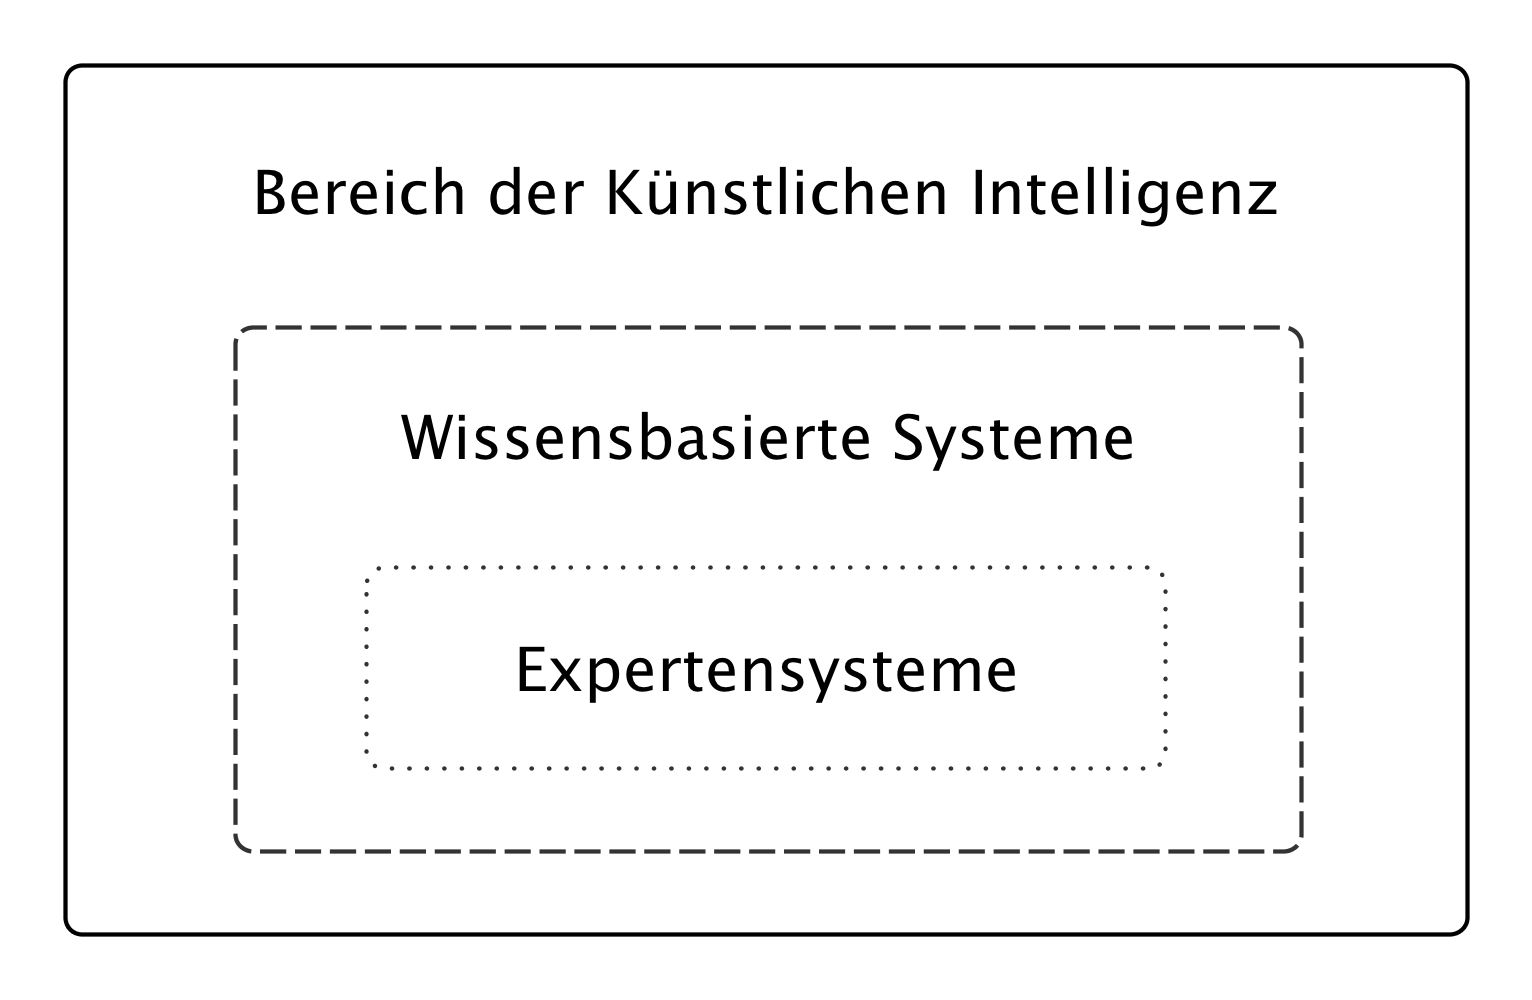
\includegraphics[width=0.55\textwidth]{images/abgrenzung.png}
	\caption{Begriffsabgrenzung, \cite[S.30]{haun2000}}
	\label{Abgrenzung}
\end{figure} 
Nach dieser Agbrenzung l�sst sich feststellen, dass der Unterschied zwischen einem Wissensbasierten System und einem Expertensystem darin besteht, dass das Wissen im Endeffekt von einem Experten stammt. Allerdings ist dieses Kriterium zu einfach und nicht besonders aussagekr�ftig. Beierle und Kern-Isberner weisen drauf hin, dass nach diesem Kriterium viele existierenden Wissensbasierten Systeme als Expertensysteme bezeichnet werden k�nnten \cite[S.11]{beierle2014}. Aufgrund dessen stellen die Autoren die Eigenschaften eines Experten dar, die sich folgenderma�en zusammenfassen lassen:
\begin{itemize}
\item Experten sind selten und teuer.
\item Experten sind nicht immer verf�gbar.
\item Leistungsf�higkeit der Experten ist nicht konstant, sondern kann nach Tagesverlauf schwanken.
\item Expertenwissen kann oft nicht als solches weitergegeben werden.
\item Expertenwissen kann verloren gehen.
\end{itemize}
Ein gutes Beispiel hinsichtlich der Gefahr, dass Expertenwissen verloren gehen kann, wird in \cite[S.94]{gebus2009} vorgestellt. Gebus nimmt den Bezug auf die Mitarbeiter der sogenannten Baby-Boomgeneration. Es handelt sich um Experten, die ein umfangreiches Erfahrungswissen besitzen und bald aus Altersgr�nden das Unternehmen verlassen. Somit geht auch das Erfahrungswissen aus dem Unternehmen verloren.\\
Zusammenfassend l�sst sich sagen, dass die Entwicklung eines Expertensystems eine hohes Potenzial besitzt. Allerdings kann ein Expertensystem nicht als Ersatz eines menschlichen Experten betrachtet werden. Vielmehr geht es um eine Erfassung, Darstellung und Pflege des Expertenwissens in einem Expertensystems, um die Arbeitsprozesse effizienter zu gestalten und sowohl erfahrene als auch neue Anwender in einem bestimmten Wissensbereich bei der Aufgabenabwicklung zu unterst�tzen.
\subsection{Architektur eines Expertensystems}\label{subsec:Architektur}
Beierle und Kern-Isberner betonen, dass die Trennung zwischen der Darstellung des Wissens in der Wissensbasis und der Wissensverarbeitung in der Wissensverarbeitungskomponente der wichtigste Aspekt eines wissensbasierten Systems ist. \cite[S.11]{beierle2014}. Die Wissensbasis kann man sich als eine Art Datenstruktur vorstellen, in der das ben�tigte Wissen gespeichert wird. Die Wissensverarbeitungskomponente umfasst eine Menge anwendungsunabh�ngiger Algorithmen, die mithilfe der Wissensbasis eine L�sung f�r ein gegebenes Problem erarbeiten. Somit stehen die Wissensbasis und die Wissensverarbeitungskomponente in einer engen Beziehung zueinander \cite[S.18]{kurbel1992}.\\
Allgemein umfasst ein Expertensystem folgende Bestandteile \cite[S.75]{greer2010}:
\begin{itemize}
\item \textit{Die Wissensbasis}, die Expertenwissen in Form von Fakten in einer bestimmten Sprache speichert, sowie Regeln zur Wissensorganisation beinhaltet.
\item \textit{Die Inferenzmaschine}, die unter Ber�cksichtigung des zugrunde liegenden Wissensbedarfs die Wissensbasis
durchsucht, bis das System einen Probleml�sungsvorschlag erarbeitet hat oder herausfindet, dass kein solcher existiert.
\item \textit{Die Dialogkomponente}, die eine Schnittstelle zwischen dem Nutzer und dem System darstellt. 
\item \textit{Die Erkl�rungskomponente}, die dem Benutzer erl�utert, warum und auf welche Weise eine bestimmte L�sung gefunden bzw. nicht gefunden wurde \cite[S.126]{haun2000}.
\item \textit{Die Wissenserwerbskomponente}, die den Entwickler des Expertensystems bei der Erweiterung, �nderung und Wartung der Wissensbasis unterst�tzt.
\end{itemize}
Laut Tecuci stellen Wissensbasis und Inferenzmaschine grundlegende Bestandteile eines Expertensystems dar und bilden damit den Kern des Expertensystems \cite[S.1444]{tecuci1992}. Dialogkomponente, Erkl�rungskomponente und Wissenserwerbskomponente geh�ren zur sogenannten Schale und sind f�r die Kommunikation zwischen dem Systemverwalter und dem Nutzer zust�ndig (siehe Abbildung \ref{expertensystem_haun}). 
\begin{figure}[H] 
	\centering
	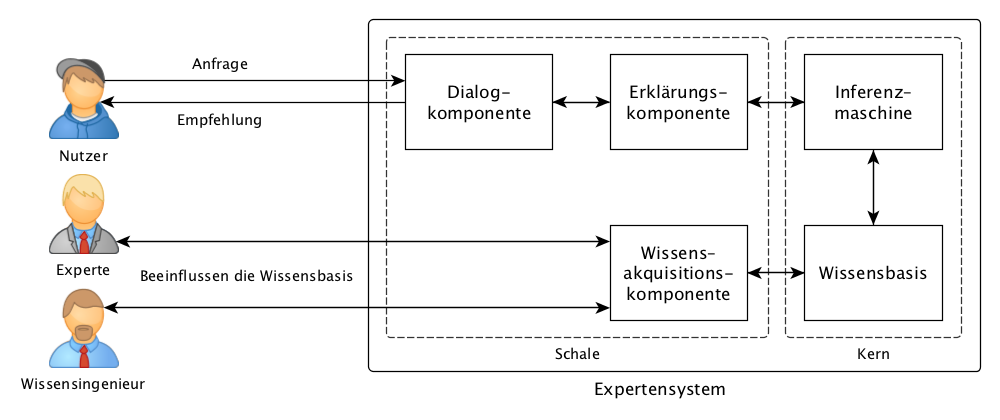
\includegraphics[width=1.0\textwidth]{images/expertensystem_haun.png}
	\caption{Expertensystem nach Haun, \cite[S.126]{haun2000}}
	\label{expertensystem_haun}
\end{figure}
Im Hinblick auf die Interaktion gibt es drei Gruppen von Personen, die mit dem Expertensystem interagieren: 
\begin{itemize}
\item \textit{Der Nutzer}, der das Expertensystem zum L�sen eines Problems benutzt und mit der Dialogkomponente kommuniziert. Der Wissensingenieur und der Experte k�nnen ebenso als Nutzer auftreten \cite[S.758]{wachsmuth1993}.
\item \textit{Der Wissensingenieur}, der sich mit dem Aufbau und der Wartung der Wissensbasis besch�ftigt. Unter anderem ist die Wissensmodellierung ein wichtiger Aufgabenbereich eines Wissensingenieurs \cite[S.742]{wachsmuth1993}.
\item \textit{Der Experte}, der �ber spezifisches Erfahrungswissen verf�gt, das f�r das Expertensystem relevant ist.
\end{itemize}
Der Ablauf der Kommunikation zwischen dem Nutzer und dem Expertensystem sieht folgenderma�en aus: 
\begin{itemize}
\item Der Nutzer schickt eine Anfrage an die Dialogkomponente des Expertensystems.
\item Die Dialogkomponente �bermittelt die Anfrage an die Inferenzmaschine.
\item Die Inferenzmaschine erarbeitet eine L�sung f�r das gegebene Problem mittels der Wissensbasis und gibt das Ergebnis an die Dialogkomponente zur�ck. 
\item Anschlie�end teilt die Dialogkomponente dem Nutzer die L�sung des Problems mit. Falls keine L�sung zum Problem existiert, wird eine entsprechende Fehlermeldung angezeigt.
\end{itemize}
Auf der anderen Seite k�nnen die Inhalte der Wissensbasis von einem Wissensingenieur mithilfe der Wissenserwerbskomponente beeinflusst werden. Der Wissenserwerb durch den Wissensingenieur ist die verbreitetste Vorgehensweise, neue Daten f�r ein wissensbasiertes System zu erschlie�en. Meistens handelt es sich um ein Interview zwischen dem Wissensingenieur und dem Experten \cite[S.76]{greer2010}, \cite[S.210]{fujihara1997}. Neben dem Interview kann der Wissensingenieur eine Recherche in den verf�gbaren Wissensquellen wie Texte, technischen Zeichnungen oder Web-Ressourcen durchf�hren. Anschlie�end formuliert der Wissensingenieur die Ergebnisse und speichert diese in der Wissensbasis.\\
Die Wissensbasis kann in einigen F�llen von Experten beeinflusst werden. Daf�r ist eine geeignete Expertenschnittstelle innerhalb der Wissenserwerbskomponente notwendig, die es den Experten erm�glicht, ihr Erfahrungswissen selbst zu formalisieren und in die Wissensbasis einzutragen \cite[S.743]{wachsmuth1993}. Die �berpr�fung des Dateninputs ist ebenfalls die Aufgabe der Wissenserwerbskomponente. Dies kann beispielsweise mittels der Durchf�hrung von automatisierten Tests erfolgen, um die Konsistenz der Wissensbasis zu gew�hrleisten \cite[S.743]{wachsmuth1993}.\\
Um ein geeignetes Konzept der automatisierten Datenerfassung zu entwickeln, ist ein grundlegendes Verst�ndnis der Struktur und Funktionsweise der Wissensbasis sowie der Wissenserwerbskomponente erforderlich. Im weiteren Verlauf der Arbeit werden deshalb die Erkenntnisse �ber die Wissensbasis und die Wissenserwerbskomponente erl�utert, die in der Forschung zu Expertensystemen entstanden sind.

\subsection{Wissensbasis}\label{subsec:Wissensbasis}
Neben der Inferenzmaschine stellt die Wissensbasis den zentralen Teil eines Ex\-per\-ten\-sys\-tems dar, der die Wissensdaten des gesamten Systems beinhaltet \cite[S.754]{wachsmuth1993}. Im Folgenden werden der allgemeine Prozess der Wissensbasisentwicklung, der Inhalt der Wissensbasis und die M�glichkeiten der Wissensrepr�sentation thematisiert. Gheorghe Tecuci beschreibt folgende Phasen bei der Entwicklung der Wissensbasis \cite[S.1444]{tecuci1992}: 
\begin{itemize}
\item Systematische Erfassung des Expertenwissens
\item Verfeinerung der Wissensbasis
\item Reorganisation der Wissensbasis
\end{itemize}
In der ersten Phase werden das Vokabular und die geeignete Wissensrepr�sentation festgelegt. Gebus und Leivisk{\"a} betonen, dass die Wissensrepr�sentation einen entscheidenden Einfluss auf die Generierung und sp�tere Handhabung der Wissensbasis hat \cite[S.95]{gebus2009}. Die initialen Daten werden meistens im Rahmen eines Interviews mit einem Experten erfasst \cite[S.1444]{tecuci1992}. Das Ergebnis der ersten Phase ist eine initiale Wissensbasis, die unvollst�ndig und teilweise widerspr�chlich sein kann. In der zweiten Phase wird die initiale Wissensbasis mithilfe geeigneter Datenerfassungsmethoden solange erweitert und verbessert, bis sie vollst�ndig und korrekt genug ist, um ein gegebenes Problem richtig zu l�sen. In der dritten Phase wird die vollst�ndige und korrekte Wissensbasis reorganisiert, um die Effizienz der L�sungsberechnung zu steigern \cite[S.1445]{tecuci1992}. Zusammenfassend werden die Phasen in Abbildung \ref{drei_phasen} dargestellt.  
\begin{figure}[H] 
	\centering
	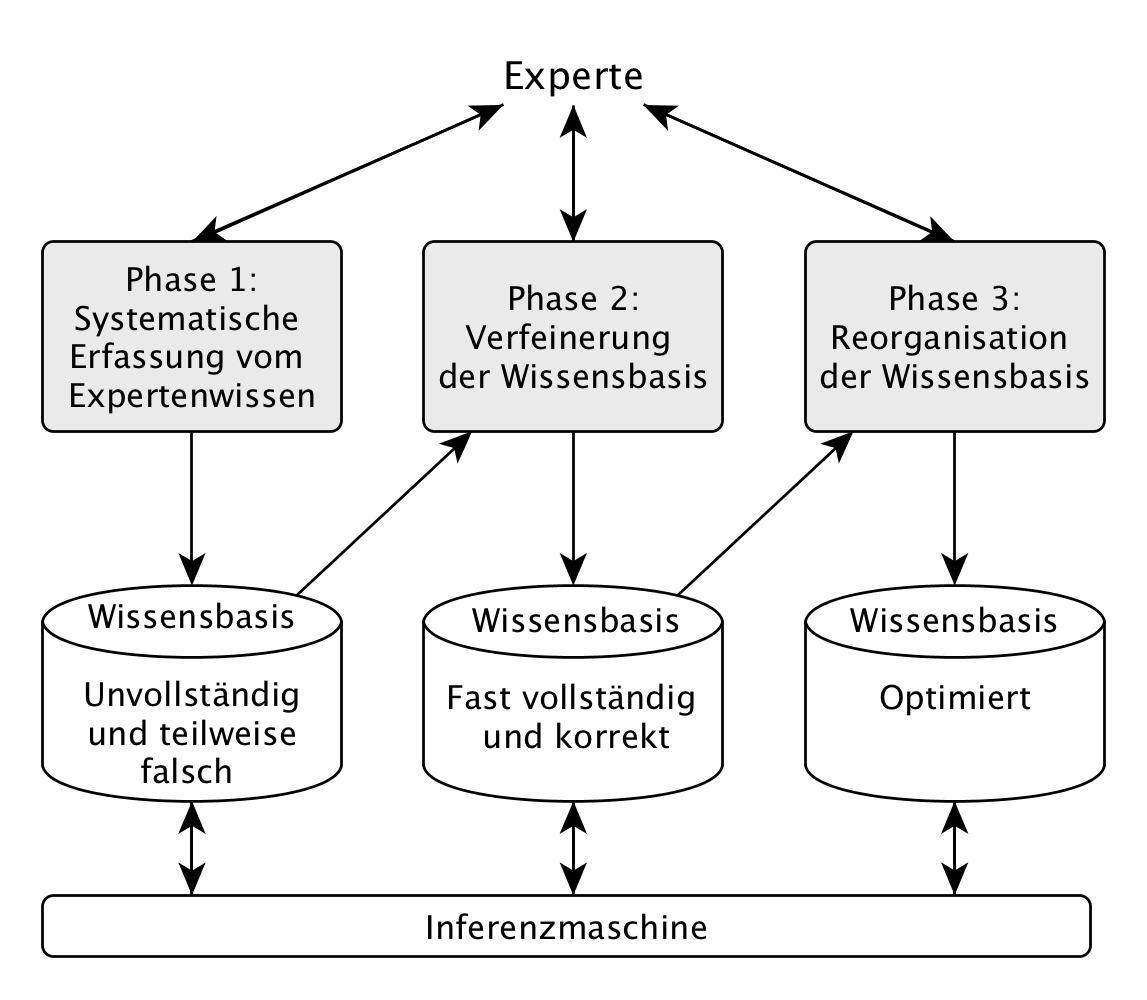
\includegraphics[width=0.7\textwidth]{images/drei_phasen.png}
	\caption{Phasen der Expertensystementwicklung, \cite[S.138]{tecuci1994}}
	\label{drei_phasen}
\end{figure}
Aus Abbildung \ref{drei_phasen} wird deutlich, dass Tecuci dem Experten die gesamte Kontrolle �ber die Entwicklung der Wissensbasis zuweist. Allerdings ist diese Sichtweise nicht vollst�ndig, da im Entwicklungsprozess der Wissensingenieur und der Systementwickler beteiligt sind und dementsprechend ber�cksichtigt werden m�ssen.\\
In Bezug auf den Inhalt der Wissensbasis unterscheiden Beierle und Kern-Isberner fol\-gende Wissensarten \cite[S.5]{beierle2014}:
\begin{itemize}
\item \textit{Fachspezifisches Wissen}: Dabei handelt es sich um das spezifische Wissen, das sich
nur auf den gerade betrachteten Problemfall bezieht. Das sind z.B. Fakten, die von Beobachtungen oder Untersuchungsergebnissen stammen.
\item \textit{Regelhaftes Wissen}: Dieses Wissen stellt den eigentlichen Kern der Wissensbasis dar und kann noch genauer differenziert werden: 
	\begin{itemize}
	\item \textit{Bereichsbezogenes Wissen}, das sich auf den gesamten Problembereich bezieht. Das kann sowohl theoretisches Fachwissen, als auch Erfahrungswissen sein.
	\item \textit{Allgemeinwissen}, das z.B. generelle Probleml�sungsheuristiken, Optimierungsregeln oder auch allgemeines Wissen �ber Objekte und Beziehungen in der realen Welt beinhaltet.
	\end{itemize}
\end{itemize}
Unter Ber�cksichtigung der Differenzierung der Wissensarten innerhalb der Wissensbasis beschreiben die Autoren in \cite[S.18]{beierle2014} auf eigene Weise die Architektur des Expertensystems, die in Abbildung \ref{expertensystem_beierle}  dargestellt wird.
\begin{figure}[H] 
	\centering
	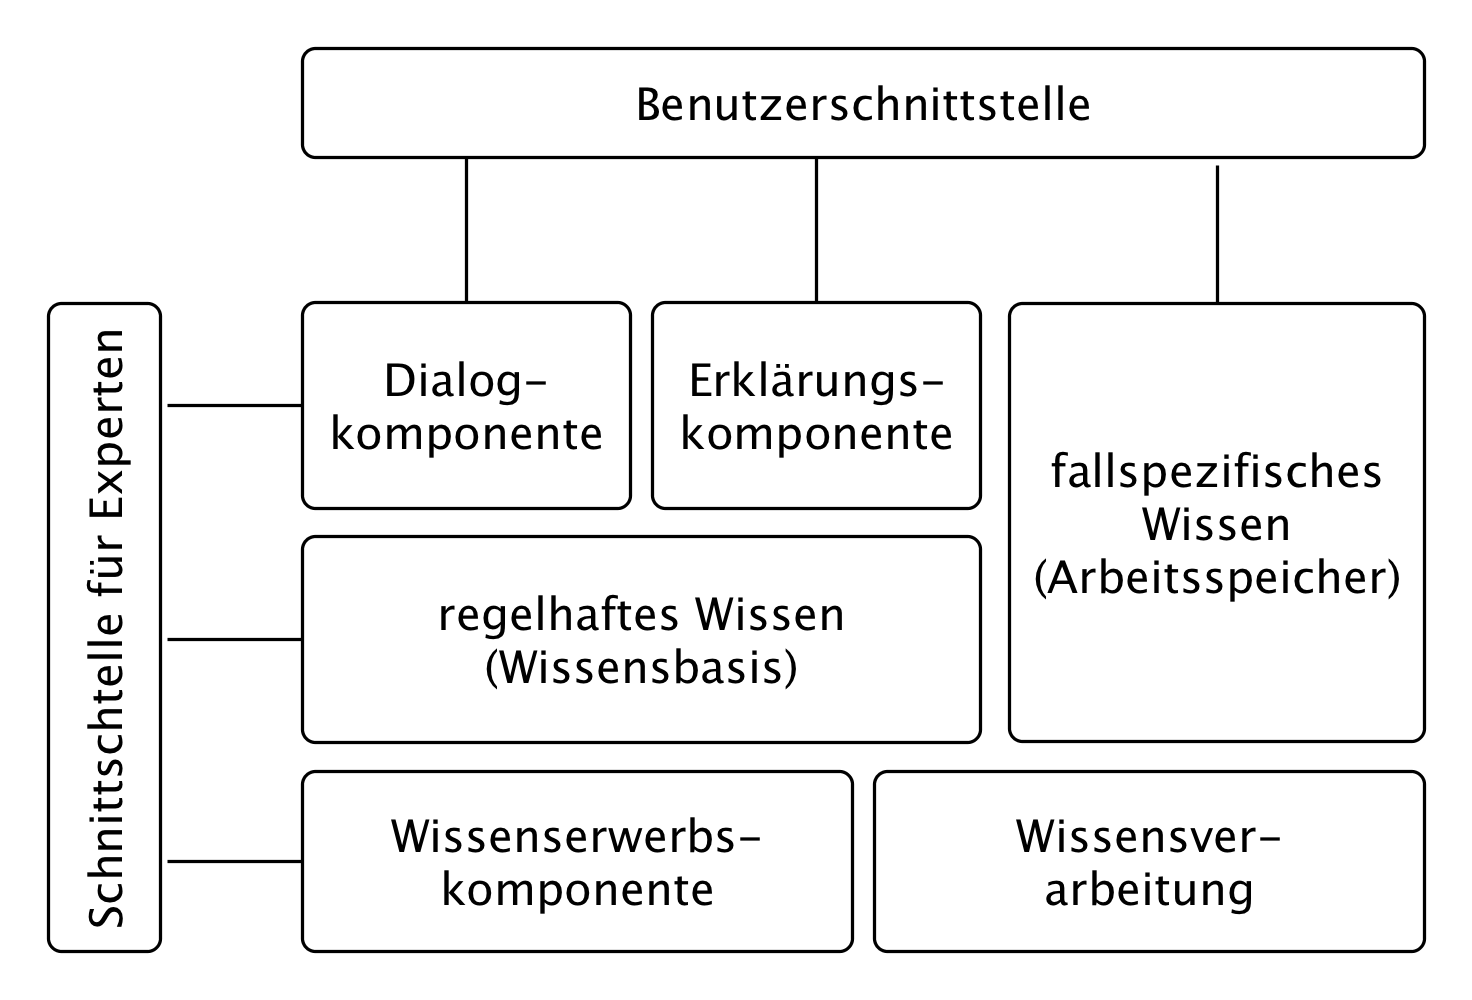
\includegraphics[width=0.70\textwidth]{images/expertensystem_beierle.png}
	\caption{Expertensystem nach Beierle und Kern-Isberner, \cite[S.18]{beierle2014}}
	\label{expertensystem_beierle}
\end{figure} 
Laut Beierle und Kern-Isberner k�nnen verschiedene Wissensarten in einem wissensbasierten System je nach dem Anwendungsbereich in unterschiedlichem Umfang auftreten. Ein hochspezialisiertes System kann beispielsweise �ber sehr wenig bis gar kein Allgemeinwissen verf�gen. Auf der anderen Seite kann ein wissensbasiertes System den Schwerpunkt auf gew�hnliches Alltagswissen legen \cite[S.5-6]{beierle2014}.\\
Ein weiterer Aspekt beim Aufbau der Wissensbasis ist die Wissensrepr�sentation. Deren grundlegende Aufgabe ist die Formalisierung von Wissen, um eine maschinelle Verarbeitung zu erm�glichen \cite[S.22]{haun2000}. Sinz und Ferstl unterscheiden folgende Formen der Wissensrepr�sentation \cite[S.366]{sinz2013}:
\begin{itemize}
\item \textit{Regelorientierte Darstellung}, in der das Wissen in Form von WENN-DANN-Regeln beschrieben wird. Diese Darstellungsform wird beispielsweise bei Prolog\footnote{F�r weitere Informationen siehe z.B. http://www.swi-prolog.org/}-Regeln eingesetzt.
\item \textit{Objektorientierte Darstellung}, die das Konzept der Objekttypen �bernimmt und mit deklarativen Operatorbeschreibungen verbindet.
\item \textit{Constraints Darstellung}, die Modellbeschreibungen aus dem Bereich des Operation Researchs benutzt. Dabei handelt es sich um L�sungsr�ume durch Neben\-be\-din\-gung\-en und Zielvorgaben.   
\end{itemize}
Hinsichtlich der Wissensrepr�sentation stellen Ferstl und Sinz imperative und deklarative Paradigmen gegen�ber \cite[S.366]{sinz2013}. Ein Programm, das dem imperativen Paradigma folgt, besteht aus einer Folge von Befehlen, die nacheinander ausgef�hrt werden \cite[S.341]{sinz2013}. Bei einem deklarativen Programm handelt es sich um eine Beschreibung der Aufgabenau�ensicht. Ein deklaratives Programm hat keine festgelegten L�sungsverfahren f�r jede Aufgabe. Stattdessen wird eine L�sung zum Zeitpunkt der Aufgabendurchf�hrung mittels Inferenzmaschine abgeleitet \cite[S.361]{sinz2013}.\\
Im Allgemeinen beziehen sich die Autoren darauf, dass an ein wissensbasiertes System nur geringe Anforderungen bez�glich Vollst�ndigkeit, Widerspruchsfreiheit und Eindeutigkeit gestellt werden k�nnen. Aus diesem Grund ist das deklarative Paradigma f�r die Wissensrepr�sentation besser geeignet. Folgende Gr�nde nennen die Autoren f�r die deklarative Umsetzung der Wissensbasis \cite[S.366]{sinz2013}: 
\begin{itemize}
\item \textit{Wissensdarstellung}: Der ein Mensch baut das Erfahrungswissen durch assoziative Beziehungsmuster auf.
\item \textit{Wissensauswertung}: �nderungen von Erfahrungswissen werden normalerweise in deklarativer Form erfasst.
\item \textit{Wissensverf�gbarkeit}: Die Codewartung eines imperativen Programms ist fehleranf�llig, sowie kosten- und zeitintensiv, da das Erfahrungswissen h�ufig ge�ndert und aktualisiert werden muss.
\end{itemize}
Der objektorientierte Ansatz ist eine weitere M�glichkeit, das Wissen zu beschreiben. Ein Beispiel f�r die objektorientierte Implementierung wird in \cite{leung1990} vorgestellt. Die Wissensbasis wird dabei als eine Sammlung von Klassen, Objekten und Methoden definiert \cite[S.40]{leung1990}. Der gro�e Vorteil einer solchen Umsetzung besteht in der Modularit�t des Wissens, d.h. das Wissen wird in unabh�ngige Module aufgeteilt. Da die einzelnen Module voneinander unabh�ngig sind, k�nnen sie getrennt getestet und modifiziert werden, ohne den Rest der Wissensbasis zu beeintr�chtigen. Dies erm�glicht eine hohe Flexibilit�t bei der Wissensbasiserweiterung \cite[S.43]{leung1990}.\\
Neben der Implementierung der Wissensbasis ist eine geeignete Umsetzung der Wissens\-erwerbskomponente erforderlich, um die Wissensbasis aktuell, m�glichst fehlerfrei und konsistent zu halten. Im Folgenden wird die Wissenserwerbskomponente in Hinsicht auf den allgemeinen Aufbau und ihre Funktionen thematisiert.  
\subsection{Wissenserwerbskomponente}\label{subsec:Wissenserwerbskomponente}
Bei der Wissenserwerbskomponente handelt es sich um einen Bestandteil des Expertensystems, der den Wissensingenieur oder einen Experten beim Aufbau und der sp�teren Erweiterung der Wissensbasis unterst�tzt \cite[S.18]{gottlob1990}. Im Allgemeinen umfasst die Wissens\-erwerbskomponente zwei grunds�tzliche Aufgaben, n�mlich den Wissenserwerb und die Pr�fung des Dateninputs auf Konsistenz, Vollst�ndigkeit und Einschr�nkungen des Expertensystems \cite[S.759]{wachsmuth1993}.\\
Unter dem Wissenserwerb wird eine �bertragung sowie Eingliederung von Wissen �ber Probleml�sungsverfahren in ein Computerprogramm verstanden \cite[S.178]{gottlob1990}. Es werden folgende Grundarten des Wissenserwerbs unterschieden \cite[S.742]{wachsmuth1993}:
\begin{itemize}
\item \textit{Indirekter Wissenserwerb}: Ein Wissensingenieur f�hrt ein Interview mit einem Experten oder einem Wissenstr�ger durch. Die Analyse der Dokumente, die f�r das System relevant sind, geh�rt ebenso zur Aufgabe des Wissensingenieurs.
\item \textit{Direkter Wissenserwerb}: Ein Wissenstr�ger gibt sein Wissen selbst mittels einer Schnittstelle in das Expertensystem ein. 
\item \textit{Automatisierter Wissenserwerb:} Die Wissensbasis wird entweder mithilfe der automatisierten Datenerschlie�ung aus verf�gbaren Dokumenten oder durch Methoden des maschinellen Lernens erweitert.
\end{itemize}
Die Methoden des indirekten Wissenserwerbs lassen sich grunds�tzlich in unstrukturierte und strukturierte Verfahren unterteilen. Das unstrukturierte Interview ist die am h�ufigsten verwendete Methode \cite[S.76]{gottlob1990}. Dabei stellt der Wissensingenieur dem Experten problembezogene Zwischenfragen, um ein m�glichst vollst�ndiges Bild des zur Probleml�sung erforderlichen Wissens zu bekommen. Die Hauptschwierigkeit bei der Wissenserhebung durch ein Interview ist die Formulierung der Fragen. Wenn die Fragen zu spezifisch sind, k�nnen wichtige Informationen ausgelassen werden \cite[S.95]{gebus2009}. Eine strukturierte Vorgehensweise der Wissenserhebung ist die Protokollanalyse, wobei der Experte beim L�sen eines Problems aufgezeichnet wird. Um den L�sungsweg nachvollziehbar zu machen, kann der Experte die Aufgabe gezielt langsamer durchf�hren oder die Aufzeichnung mit Kommentaren versehen. Die aufgabenbezogenen L�sungen werden mithilfe von Induktion generalisiert. Bei der Induktion wird eine allgemeine Regel aus den Einzelf�llen abgeleitet \cite[S.308]{castro2001}. Anschlie�end werden die erzielten Ergebnisse vom Wissensingenieur formalisiert und ins Expertensystem eingetragen.\\
Beim direkten Wissenserwerb soll eine geeignete Schnittstelle im Rahmen der Wissenserwerbskomponente zur Verf�gung gestellt werden, die es dem Wissenstr�ger erm�glicht, sein Wissen ins System einzugeben. Die Schnittstelle soll eine dem Wissenstr�ger bekannte Wissensrepr�sentation verwenden und benutzerfreundlich sein \cite[S.743]{wachsmuth1993}. Ein Beispiel f�r Benutzerfreundlichkeit ist die gleichzeitige Validierung der Benutzereingaben sowie eine R�ckmeldung bei unzul�ssigen Aktionen. Der direkte Wissenserwerb hat den Vorteil, dass die Wissensbasis ohne den Wissensingenieur erweitert werden kann. Allerdings betonen die Autoren in \cite[S.765]{wachsmuth1993}, dass dies nur in gut verstandenen und strukturierten Anwendungsbereichen m�glich sei.\\
Bez�glich des automatisierten Wissenserwerbs gibt es wenige Erkenntnisse, die allgemein anwendbar sind. Meistens handelt es sich um L�sungen, die nur innerhalb eines spezifischen Anwendungsbereichs funktionieren. Nichtsdestotrotz l�sst sich sagen, dass sich das Wissen entweder aus vorhandenen Daten durch maschinelles Lernen oder aus verf�gbaren Dokumenten durch automatisierte Dokumentenanalyse generieren l�sst \cite[S.78]{gottlob1990}. Die Implementierung h�ngt jedoch vom Anwendungsgebiet ab. Ein Beispiel f�r die Anwendung maschinellen Lernens auf gro�e Datenmengen ist ein Diagnosesystem, das f�r eine Vielzahl von F�llen mit bestimmten Symptomen Diagnosen enth�lt. F�r die Textanalyse k�nnen beispielsweise Bedienungsanleitungen analysiert werden, wobei diese Vorgehensweise gewisse Einschr�nkungen aufweist. Die Schwierigkeit besteht darin, dass das Erfahrungswissen nicht in den Textdokumenten zu finden ist \cite[S.79]{gottlob1990}.\\
In allen F�llen des Wissenserwerbs werden die Daten an die zentrale Schnittstelle weitergereicht. Diese besch�ftigt sich mit der Zwischenspeicherung und der Pr�fung der Datens�tze auf Korrektheit, bevor die Daten endg�ltig in der Wissensbasis gespeichert werden. Zum Teil kann der Wertebereich direkt im einzelnen Modul des Wissenserwerbs eingeschr�nkt werden. Beispielsweise kann ein Eingabefeld in der Wissenstr�gerschnittstelle nur positive Zahlen zulassen. F�r den restlichen Teil werden automatisierte Tests durchgef�hrt, die sicherstellen, dass neue Daten keine Inkonsistenzen in Bezug auf die Einschr�nkungen der Wissensbasis erzeugen \cite[S.765]{wachsmuth1993}.\\
Zusammenfassend l�sst sich die Wissenserwerbskomponente schematisch wie in Abbildung \ref{fig:wissenserwerbskomponente} wie folgt darstellen:
\begin{figure}[H] 
	\centering
	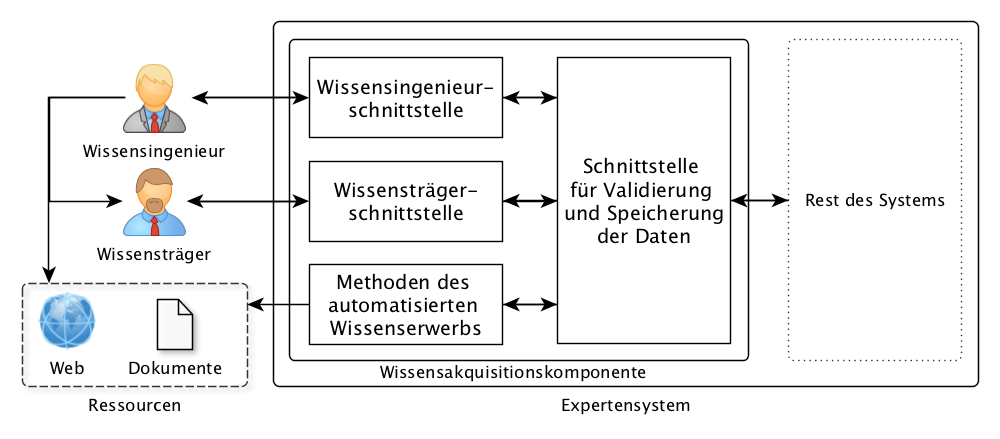
\includegraphics[width=0.9\textwidth]{images/wissenserwerbskomponente.png}
	\caption{Wissenserwerbskomponente}
	\label{fig:wissenserwerbskomponente}
\end{figure}
Daraus wird deutlich, dass die Wissenserwerbskomponente modular aufgebaut ist. Allgemein kann dieses Modell in jedem Expertensystem eingesetzt werden, wobei die konkrete Umsetzung in Bezug auf den Anwendungsbereich spezifiziert wird. Dabei l�sst sich der Automatisierungsgrad der Datenerfassung leicht anpassen, indem der Schwerpunkt auf ausgew�hlte Bestandteile der Wissenserwerbskomponente gelegt wird. Beispielsweise kann sich ein Expertensystem mit umfangreichen Falldaten auf das maschinelle Lernen konzentrieren. Ein System, das bei der Datenerfassung mithilfe der Wissenstr�gerschnittstelle basiert, wird in \cite[S.97]{gebus2009} vorgestellt.\\
Im weiteren Verlauf der Arbeit werden die Wissenstr�gerschnittstelle, die Methoden des automatisierten und halb-automatisierten Wissenserwerbs sowie die Schnittstelle zur Daten�bermittlung thematisiert, da sie Potenzial f�r die Automatisierung der Da\-ten\-er\-fas\-sung aufweisen.
\newpage
\section{Methoden der Wissens- und Datenerfassung}\label{sec:Wissenserfassung}
Mit der Wissenserwerbskomponente wurde bereits angedeutet, dass die Erweiterung bzw. Aktualisierung der Wissensbasis eines Expertensystemes meistens nur teilweise automatisierbar ist. Die Autoren in \cite{tecuci1994} weisen ebenso darauf hin, dass manuelle und maschinelle Wissenserschlie�ung jeweils eigene St�rke haben, die sich gegenseitig erg�nzen  \cite[S.137]{tecuci1994}. Aus diesem Grund ist bei der Datenerfassung ein hybrides Modell sinnvoll, das die Vorteile manueller und maschineller Verfahren kombiniert. Aufgrund der Fragestellung dieser Arbeit wird es im Weiteren auf automatisierte und halb-automatisiere Bestandteile der Wissenserwerbskomponente beschr�nkt.
\subsection{Schnittstelle zur Dateneingabe}
Die Schnittstelle zur Dateneingabe (auch als Wissenstr�gerschnittstelle in Kapitel \ref{subsec:Wissenserwerbskomponente} beschrieben) ist in der Regel ein Bestandteil eines Tools zum Wissenserwerb. Diese Schnittstelle soll dem Wissenstr�ger erm�glichen, sein Wissen auf eine einfache Weise in das System einzutragen. Da die Daten manuell eingegeben und maschinell verarbeitet werden, wird dieser Ansatz als semi-automatisiert bezeichnet. Im Zusammengang mit der Wissenstr�gerschnittstelle wurden zahlreiche Tools entwickelt (z.B. in \cite{rafea2003} oder \cite{gebus2009}), die sich in Automatisierungsgrad, Problembereich oder Benutzergruppe unterscheiden \cite[S.49]{rafea2003}. Im Folgenden wird eine Arbeit genauer betrachtet, die den Einsatz der Wissenstr�gerschnittstelle beispielhaft darstellt.\\
Das Praxisbeispiel wird in \cite{gebus2009} vorgestellt und bezieht sich auf die Wissenserfassung aus der Produktion eines Elektrotechnikunternehmens. In der Fallstudie wird ein bereits bestehendes \acf{DSS} betrachtet, das die F�hrungskr�fte bei der Entscheidung nicht-strukturierter Probleme in der Produktion unterst�tzt \cite[S.94]{gebus2009}. Das DSS verf�gt bereits �ber eine Datenbank, die allerdings nur Daten von Produkteigenschaften enth�lt. Die eigentlichen Prozesse werden hierbei von Experten gesteuert, die mithilfe ihres Erfahrungswissens St�rungen in der Produktion beseitigen. Dieses Erfahrungswissen �ber St�rungen wird im System nicht erfasst. Als Folge hat die Unternehmensf�hrung nur einen begrenzten �berblick �ber die Situation in der Produktionsabteilung. Au�erdem besteht die Gefahr, dass das spezifische Expertenwissen verloren geht, falls der Wissenstr�ger das Unternehmen verl�sst \cite[S.467]{song2016}.\\
Die Zielsetzung von \cite{gebus2009} ist die Erfassung des Expertenwissens aus der Produktion und die Integration dieses Wissens in die Entscheidungsprozesse auf der Organisationsebene. Um das Wissen aus der Produktionsabteilung zu erschlie�en, erweitern Gebus und Leivisk{\"a} das bestehende System um eine Schnittstelle f�r Anlagenbediener. Die Umsetzung erfolgt in Form eines Prototyps. Der Entwicklungsprozess l�sst sich allgemein wie folgt beschreiben:
\begin{itemize}
\item[1.] Die Definition der Zielgruppe, die f�r die Schnittstelle relevant ist.
\item[2.] Ausgehend von der Zielgruppe werden die Wissensrepr�sentation sowie funktionale und nicht-funktionale Anforderungen spezifiziert.
\item[3.] Die Umsetzung und Evaluation des Prototyps.
\end{itemize}
Im ersten Schritt definieren Gebus und Leivisk{\"a} die bestehenden Nutzergruppen des gesamten Systems \cite[S.97]{gebus2009}:
\begin{itemize}
\item Anlagenbediener (Experte), der sein Wissen zu den St�rungen mittels der Wissenstr�gerschnittstelle in die Datenbank eingibt,
\item Administrator, der das gesamte System verwaltet,
\item Qualit�tsabteilung, die die St�rungsstatistik analysiert, eine Qualit�tsr�ckmeldung an die Produktion und einen Bericht an die F�hrungskraft �bermittelt,
\item F�hrungskraft, die eine umfangreiche �bersicht von der Qualit�tsabteilung erh�lt und davon ausgehend Entscheidungen zur Prozessoptimierung trifft.
\end{itemize}
Im Rahmen der Fallstudie ist die Nutzergruppe der Anlagenbediener relevant, wobei das System jeder Nutzergruppe eine geeignete Benutzerschnittstelle zur Verf�gung stellt. Schematisch l�sst sich die Struktur und die Informationsfl�sse im DSS in Abbildung \ref{dss_gebus} vereinfacht nachbilden.
\begin{figure}[H] 
	\centering
	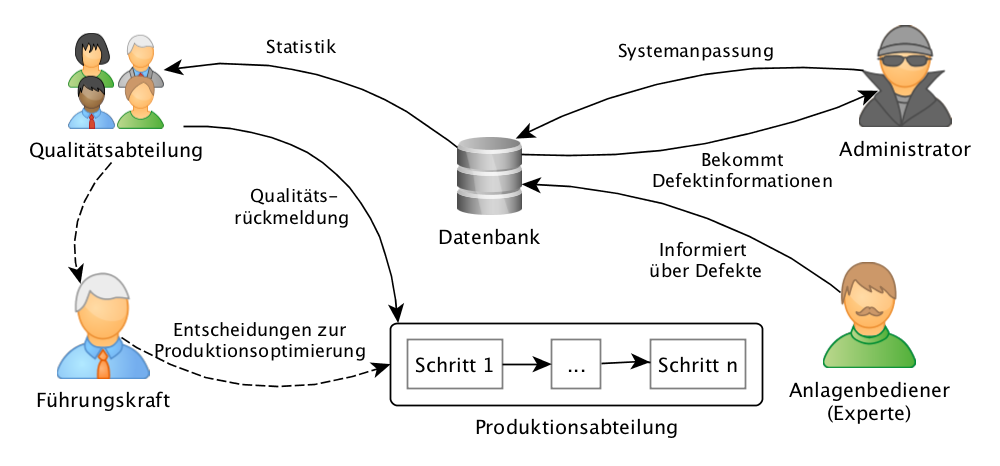
\includegraphics[width=0.95\textwidth]{images/dss_gebus.png}
	\caption{Die Struktur und die Informationsfl�sse im DSS, \cite[S.98]{gebus2009}}
	\label{dss_gebus}
\end{figure} 
F�r die Informationsrepr�sentation werden die Anlagenbilder benutzt. Die Autoren betonen, dass die Expertenschnittstelle so einfach und intuitiv wie m�glich gehalten wurde, um die Dateneingabe zu einer allt�glichen T�tigkeit zu machen \cite[S.97]{gebus2009}. Im Hinblick auf die nicht-funktionalen Anforderungen werden beispielsweise Einstellungen und Maschinenbilder vom Administrator vorkonfiguriert und automatisch beim Hochfahren des Systems geladen. Die funktionalen Anforderungen umfassen die Erfassung einer St�rung durch die Auswahl des passenden Anlagebildes und das Markieren der betroffenen Stelle. Darauffolgend wird eine Vorlage mit m�glichen Ursachen zur Auswahl angezeigt. Zus�tzlich gibt es ein Feld zur Freitexteingabe, wenn die vorliegende St�rung im System noch nicht vorhanden ist \cite[S.99]{gebus2009}.\\
In der Evaluation haben sich folgende benutzerorientierte Kriterien f�r die weitere Systemverbesserung ergeben \cite[S.100]{gebus2009}:
\begin{itemize}
\item \textit{Usability (engl. Gebrauchstauglichkeit)}: Wie einfach und intuitiv ist das System zu verwenden.
\item \textit{Usefulness (engl. N�tzlichkeit)}: Wie n�tzlich ist das System f�r prim�re (Anlagenbediener) und sekund�re (z.B. Qualit�tsabteilung) Nutzer.
\item \textit{Usage (engl. Nutzung)}: Inwiefern wird das System verwendet.
\end{itemize}
Wenn es um die Benutzerinteraktion mit einem System geht, spielt Usability die zentrale Rolle. Gem�� ISO 9241-11 wird Usability durch folgende Aspekte definiert: Effektivit�t (wurde das Ziel erreicht), Effizienz (wie schnell wurde das Ziel erreicht) und Zufriedenheit (positive Erfahrung bei der Systemnutzung) \cite{iso9241}. Usefulness wird in \cite{krug2014} behandelt. Steve Krug bezeichnet einen Gegenstand als n�tzlich, wenn eine Person mit durchschnittlichen F�higkeiten herausfinden kann, wie dieser Gegenstand zu bedienen ist, um ein Ziel zu erreichen. Dabei soll der Aufwand kleiner als der Wert des Ziels sein \cite[S.9]{krug2014}.\\
Statistisch gesehen gab es in der betrachteten Testperiode 183 Anlagenausf�lle. Allerdings wurden nur 70 F�lle kommentiert, was eine Nutzungsrate des vorgestellten Informationsaustauschsystems von 38\% ergibt. Laut Gebus und Leivisk{\"a} lag es daran, dass der Prototyp aus der Usability-Perspektive nicht optimal war. Beispielsweise waren einige Elemente der Schnittstelle eher verwirrend. Nach den notwendigen Anpassungen konnte die Nutzungsrate fast auf 100\% gesteigert werden. Hinsichtlich der N�tzlichkeit gab es positive Bewertungen. Es wurde festgestellt, dass die Umwandlung des Systems aus einer reinen Datensammlung �ber St�rungen zu einem Informationsaustauschsystem Vorteile f�r alle Nutzergruppen bringt. In Abbildung \ref{dss_gebus} sieht man deutlich, dass die Informationen, die in der Datenbank gespeichert werden, von allen Beteiligten genutzt werden. Der Administrator kann mithilfe der Daten das System entsprechend anpassen. Die Qualit�tsabteilung setzt die Information zur Berichterstellung f�r die F�hrungskr�fte und die Produktion ein. Die Unternehmensf�hrung erh�lt ein umfangreicheres Bild �ber die Produktionslage und kann aufgrund dessen effizientere Entscheidungen bei der Produktionsoptimierung treffen. \\
Zusammenfassend l�sst sich sagen, dass die Entwicklung der Wissenstr�gerschnittstelle aus drei Phasen besteht. In der ersten Phase wird die Zielgruppe definiert. Im Hinblick auf die Zielgruppe werden in der zweiten Phase die geeignete Informationsrepr�sentation sowie die funktionalen und nicht-funktionalen Anforderungen festgelegt. Die dritte Phase umfasst die Implementierung mit der darauffolgenden Evaluation, in dem die Schnittstelle nach drei Kriterien bewertet wird, n�mlich Usability, Usefulness und Usage.


\subsection{Datenerfassung aus dem Web}\label{subsec:webdaten}
Der Prozess der Webdatenerfassung umfasst die Datenextraktion aus unstrukturierten bwz. semi-strukturierten Webdokumenten (z.B. eine Webseite oder eine E-Mail) und die Transformation der erfassten Daten in eine strukturierte Form zur sp�teren Verwendung \cite[S.301]{ferrara2014}. Im Folgenden werden die allgemeinen Probleme bei der Erfassung von Webdaten angesprochen. Anschlie�end werden generelle Paradigmen der Datenerfassung erl�utert, n�mlich das Baumparadigma, Web-Wrapper und hybride Systeme.\\
Bei der Erfassung der Webdaten gibt es mehrere Faktoren, die ber�cksichtigt werden sollen. Ferrara et al. \cite[S.302]{ferrara2014} identifizieren folgende Herausforderungen:
\begin{itemize}
\item \textit{Automatisierungsgrad}: Die Erfassung der Webdaten soll regelm��ig von einem menschlichen Experten �berwacht werden, um die Genauigkeit der Daten zu gew�hrleisten.
\item \textit{Skalierbarkeit}: Bei umfangreichen Webressourcen soll innerhalb kurzer Zeit eine gro�e Datenmenge bearbeitet werden.
\item \textit{Datenschutz}: Wenn es um die Erfassung personenbezogener Daten geht (z.B. bei sozialen Netzwerken wie Facebook), soll die Privatsph�re des Individuums nicht beeintr�chtigt werden.
\item \textit{�nderung der Ressourcenstruktur}: Die Struktur von Webressourcen �ndert sich oft. Die Datenerfassungsmethoden f�r das Web sollen eine gewisse Flexibilit�t besitzen, um weiterhin korrekt zu funktionieren.
\item \textit{Trainingsdaten}: Beim Einsatz des maschinellen Lernens ist eine ausreichende Trainingsmenge an Webseiten erforderlich, die manuell vorbereitet wird. Dies ist eine aufwendige und fehleranf�llige Aufgabe.
\end{itemize}
Das Baumparadigma nutzt die Baumstruktur einer Webseite, um die gew�nschten Daten zu erfassen. Dabei handelt es sich um Dokumente, die in der \acf{HTML} beschrieben sind. Eine HTML-Seite wird als \acf{DOM}\footnote{https://www.w3.org/DOM} definiert. Die Idee des DOM besteht darin, dass eine HTML-Webseite in einer Baumstruktur dargestellt wird, die mittels HTML-Tags (z.B. Button-Tag) ausgezeichnet ist. Tags k�nnen weitere Tags beinhalten und bilden somit eine hierarchische Struktur, die eine effiziente Datensuche auf einer HTML-Seite erm�glicht \cite[S.303]{ferrara2014}.\\
Da HTML Eigenschaften einer \acf{XML} integriert, kann die \acf{XPath}\footnote{https://www.w3.org/TR/xpath} zur Navigation im DOM eingesetzt werden. In einem XPath-Ausdruck k�nnen beliebige Elemente einer HTML-Webseite ausgew�hlt werden. In Abbildung \ref{xpath} werden zwei Beispiele dargestellt. Im ersten Fall (A) wird genau ein Element einer Tabelle (die erste Zelle in der ersten Zeile) ausgew�hlt. Im Beispiel (B) werden mehrere Elemente (alle Zellen der zweiten Zeile) angesprochen \cite[S.303]{ferrara2014}.
\begin{figure}[H] 
	\centering
	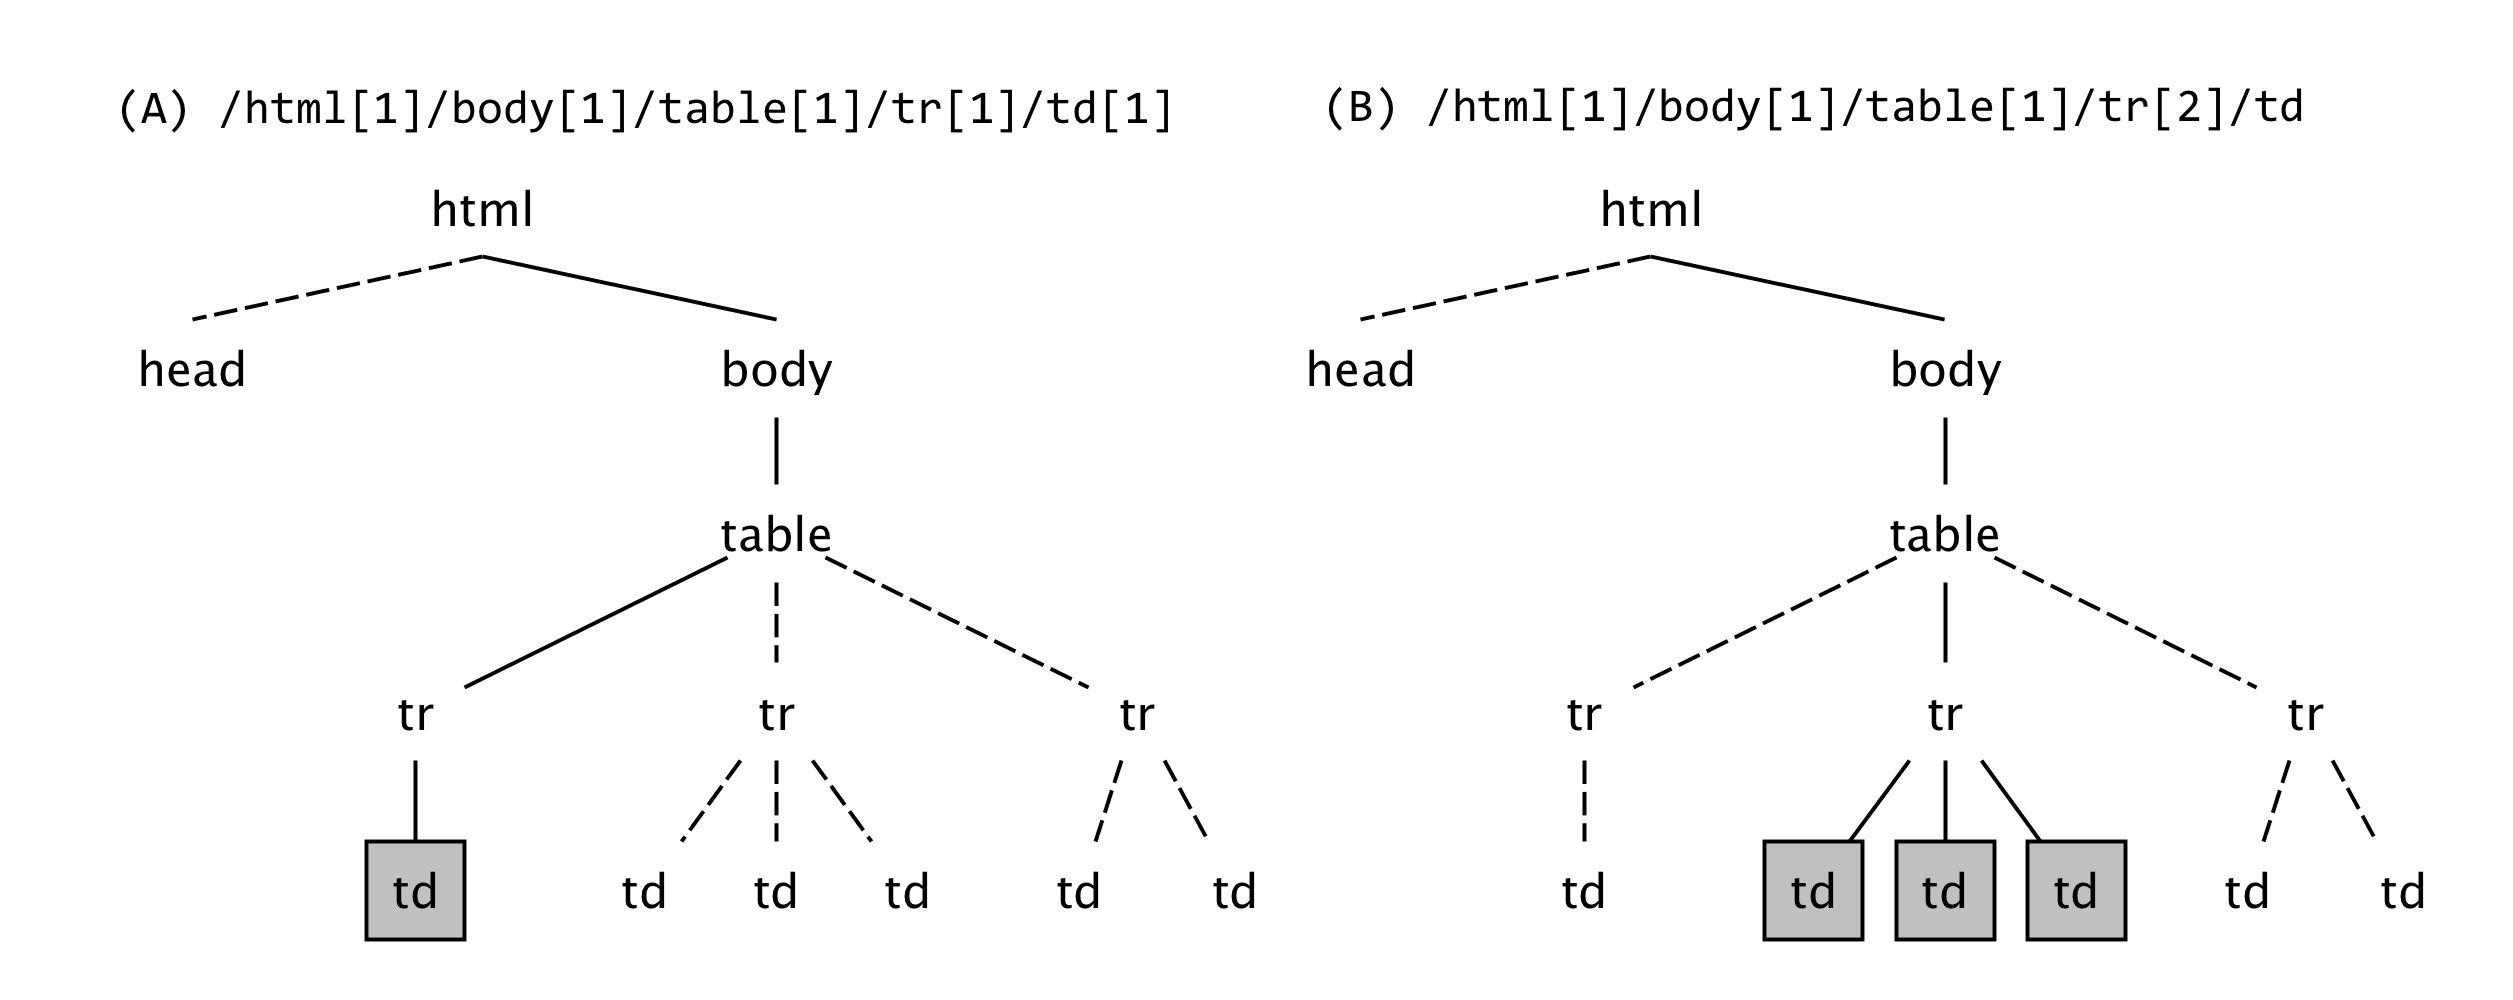
\includegraphics[width=1.0\textwidth]{images/xpath.png}
	\caption{XPath im Dokumentenbaum, \cite[S.304]{ferrara2014}}
	\label{xpath}
\end{figure} 
Der gr��te Nachteil von XPath besteht darin, dass XPath-Ausdr�cke strikt an die DOM-Struktur gebunden sind. Wenn eine �nderung im DOM stattfindet, funktioniert der von der �nderung betroffene Ausdruck nicht mehr. Aus diesem Grund m�ssen die XPath-Ausdr�cke nach jeder Ver�nderung der HTML-Webseite manuell angepasst werden. Hinsichtlich dieses Problems wurden im letzten Release von XPath\footnote{https://www.w3.org/TR/xpath20} relative XPath-Ausdr�cke eingef�hrt \cite[S.304]{ferrara2014}.\\
Ein weiterer Ansatz, die Webdaten zu erfassen, stellt ein Web-Wrapper dar. Dieser umfasst in der Regel einen oder mehrere Algorithmen, die zur Datenerfassung aus den Webdokumenten eingesetzt werden. Anschlie�end werden die erfassten Daten in eine strukturierte Form transformiert und f�r die weitere Nutzung gespeichert. Ein Web-Wrapper umfasst folgende Schritte \cite[S.305]{ferrara2014}:
\begin{itemize}
\item[1.]\textit{Generierung}: Definition des Wrappers.
\item[2.]\textit{Ausf�hrung}: Datenerfassung mithilfe des Wrappers.
\item[3.]\textit{Wartung}: Anpassung des Wrappers bei der �nderung der DOM-Struktur.
\end{itemize}
Nach Ferrara et al. \cite[S.306]{ferrara2014} kann ein Web-Wrapper mittels folgender Ans�tze generiert und ausgef�hrt werden:
\begin{itemize}
\item \textit{Regul�re Ausdr�cke}: Daten werden gem�� Regeln (expressions) gewonnen. Im Rahmen dieser Arbeit wird sich auf diesen Ansatz der regul�ren Ausdr�cke beschr�nkt.
\item \textit{Logikbasierter Ansatz}: Zur Datenerfassung wird eine Wrapper-Programmiersprache eingesetzt (wrapper programming language).
\item \textit{Baumbasierter Ansatz}: Es wird die Annahme getroffen, dass bestimmte Bereiche im DOM generell f�r Daten zust�ndig sind. Die Identifikation und Datenextraktion aus diesen Bereichen ist der Gegenstand des baumbasierten Ansatzes.  
\item \textit{Maschinelles Lernen}: Daten werden mithilfe eines Lernalgorithmus und einer Trainingsmenge erfasst.
\end{itemize} 
Regul�re Ausdr�cke erm�glichen die Erkennung von Mustern in unstrukturierten bzw. semi-strukturierten Dokumenten unter Verwendung von Regeln, die z.B. in Form von Wortgrenzen oder HTML-Tags definiert werden. Der Vorteil der regul�ren Ausdr�cke besteht in der M�glichkeit, ein beliebiges Element auf einer Webseite anzusprechen. Au�erdem bieten einige Implementierungen ein grafisches Benutzerinterface, sodass der Benutzer die Elemente auf einfache Weise ausw�hlen kann. Die f�r die Erkennung ben�tigten Regeln werden dann automatisch generiert. Eine m�gliche Umsetzung des Wrappers wird in \cite{sahuguet1999} mit W4F vorgestellt. Dieses Tool verf�gt �ber eine Hilfsmethode, die den Benutzer bei der Auswahl der Elemente unterst�tzt. Auf Basis der ausgew�hlten Elemente werden die Regeln erstellt. Allerdings sind die Regeln in Bezug auf DOM-�nderungen nicht flexibel und k�nnen sehr schnell verletzt werden \cite[S.306]{ferrara2014}.\\
In der dritten Phase geht es um die Anpassung des Web-Wrappers im Hinblick auf Ver�nderungen der DOM-Struktur. Die Anpassung erfolgt entweder manuell oder zum Teil automatisiert. Ferrara et al. \cite[S.308]{ferrara2014} betonen, dass der Automatisierungsgrad der Wartung besonders kritisch ist. Bei einer kleinen Dokumentenanzahl ist die manuelle Anpassung noch akzeptabel. Allerdings ist die manuelle Wartung bei einer gro�en Menge von Dokumenten nicht mehr realisierbar.\\
Ein Beispiel der automatisierten Wrapper-Wartung wird in \cite{meng2003} mit dem System namens SG-WRAM (Schema-Guided Wrapper Maintenance for Web-Data Extraction) vorgestellt. Die Architektur von SG-WRAM wird in Abbildung \ref{wram} dargestellt.
\begin{figure}[H] 
	\centering
	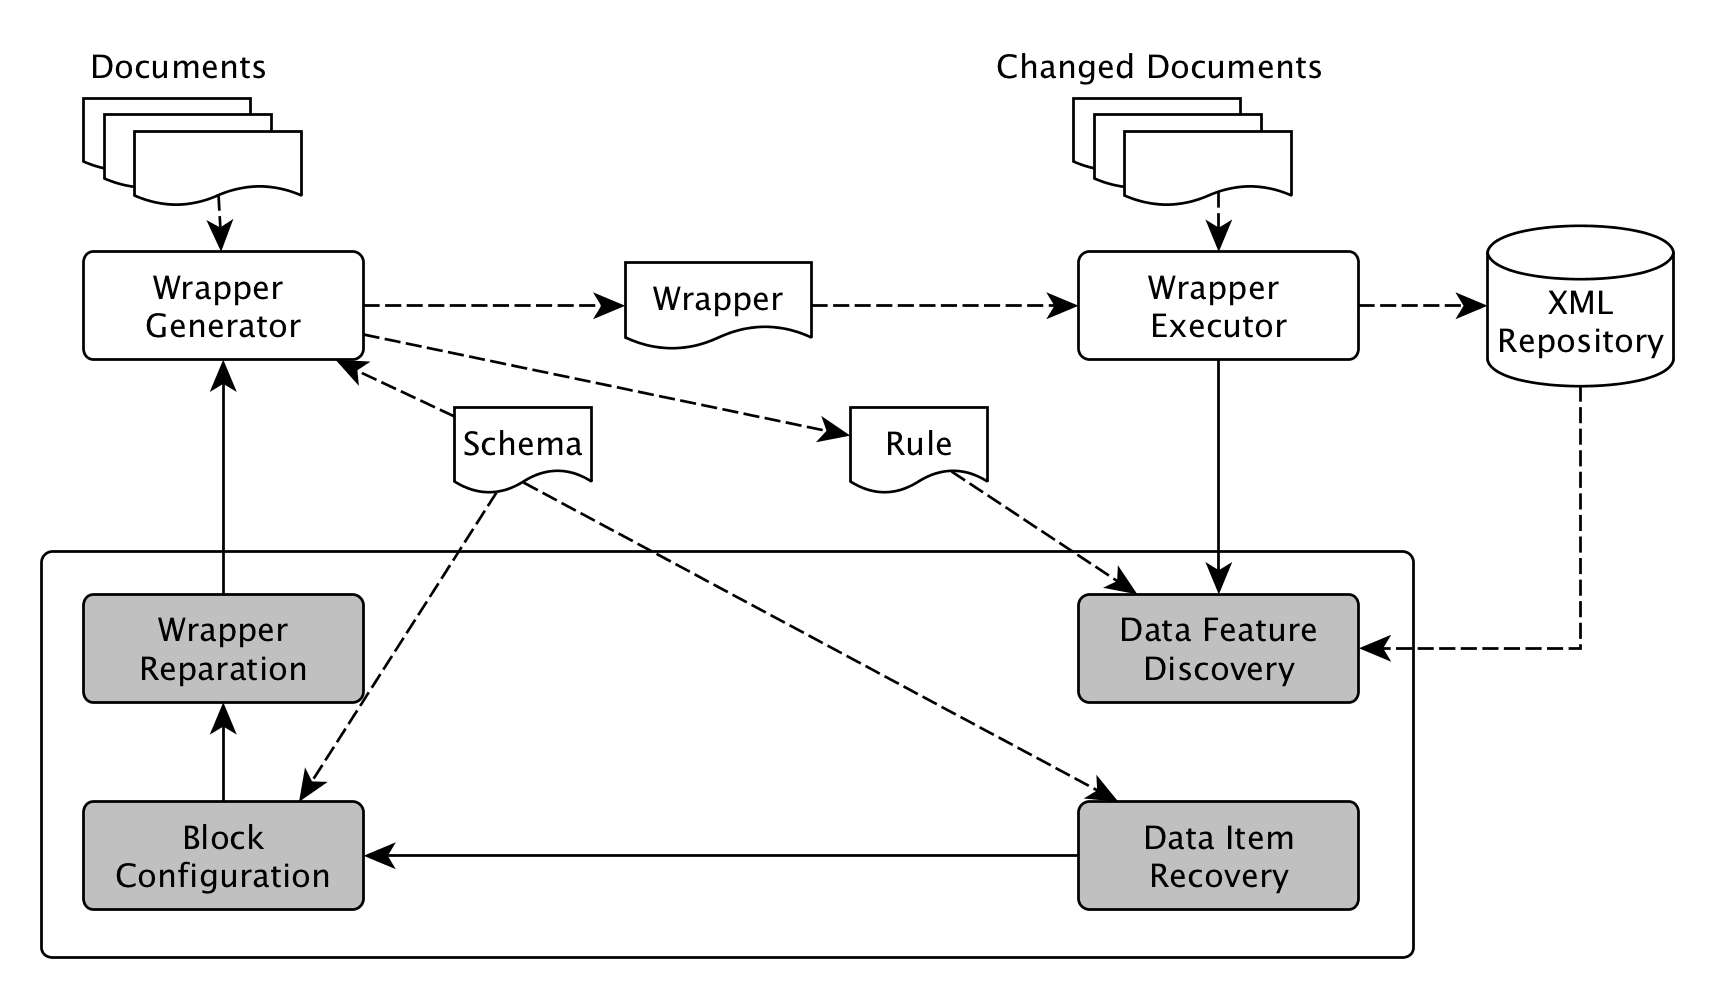
\includegraphics[width=1.0\textwidth]{images/wram.png}
	\caption{Die Architektur von SG-WRAM, \cite[S.2]{meng2003}}
	\label{wram}
\end{figure} 
Im ersten Schritt werden die HTML-Seite, das XML-Schema und das Mapping zwischen diesen in den Wrapper-Generator eingegeben. Das XML-Schema wird durch eine \acf{DTD} beschrieben. Daraufhin generiert das System die Regeln (Wrapper) f�r die gegebene Webseite, um die Daten zu erfassen und in einer XML-Datei gem�� der DTD zu speichern. Neben der Datenextraktion werden zus�tzlich die Probleme bei der Extraktion erfasst, um ein Wiederherstellungsprotokoll f�r fehlgeschlagene Regelerzeugungen zu generieren. Wenn das Protokoll die Fehler beseitigt, wird die Datenerfassung fortgesetzt. Bei auftretenden Fehlern werden Warnungen und Benachrichtigungen angezeigt, dass die Regeln nicht mehr funktionieren. In diesem Fall m�ssen die Regeln manuell von einem Experten angepasst werden \cite[S.308]{ferrara2014}.\\
Als Ausblick wird ein hybrides System der Webdatenerfassung angesprochen. Ein Beispiel des hybriden Ansatzes ist RoadRunner von \cite{crescenzi2001}. Dies kann sowohl mit der Trainingsmenge eines Nutzers als auch mit selbst erstellten Trainingsdaten ausgef�hrt werden. Das Verfahren arbeitet gleichzeitig mit zwei HTML-Seiten und analysiert die Gemeinsam\-keit\-en und die Unterschiede zwischen diesen, um die Muster zu finden. Im Allgemeinen kann das Verfahren die Daten aus beliebigen Quellen erfassen, solange mindestens zwei Seiten mit �hnlicher Struktur gegeben sind. Da Webseiten normalerweise dynamisch auf Basis eines Templates generiert werden, befinden sich relevante Daten in gleichen oder �hnlichen Bereichen \cite[S.309]{ferrara2014}.
\subsection{Maschinelles Lernen beim Wissenserwerb}\label{subsec: Maschinelles-Lernen}
In diesem Abschnitt handelt es sich um einen Ausblick in weitere Wissenserwerbsmethoden, und zwar die Anwendung des maschinellen Lernens. In der Literatur gibt es eine Reihe der Ans�zte, die sich damit besch�ftigen (z.B. \cite{castro2001} und \cite{webb1996}). Trotz der Unterschieden in der Umsetzung gibt es eine entscheidende Gemeinsamkeit. Beide Methoden basieren auf der Zusammenarbeit zwischen dem Experten und dem Lernalgorithmus. Im Folgenden wird der Ansatz von \cite{castro2001} genauer betrachtet.\\
In der Arbeit von \cite{castro2001} handelt es sich um die Anwendung des maschinellen Lernens bei der Erfassung des Expertenwissens im Medizinbereich. Das Konzept der Wissensbasiserweiterung orientiert sich an \cite{tecuci1992} und besteht darin, dass anfangs eine initiale Wissensbasis gebaut und inkrementell verbessert wird, indem der Experte die Fragen vom System beantwortet. Bei der Erstellung der Fragen wird ein Lernverfahren eingesetzt. Die Idee des Lernverfahrens besteht in der Erschlie�ung des naheliegenden Expertenwissens aus den Trainingsdaten der Schlussfolgerungen eines Experten.\\
Der Kern des Verfahrens besteht aus dem induktiven Lernen und dem generischen Algorithmus von \cite{castro1999}, der auf der Fuzzylogik basiert ist. Bei der Induktion handelt es sich um das Erschlie�en der allgemeinen Schlussfolgerungen aus den Einzelf�llen. Die Fuzzylogik besch�ftigt sich mit den graduellen Aussagen, die nicht eindeutig falsch oder wahr bezeichnet werden k�nnen. Diese Aussagen werden mithilfe der vagen Pr�dikaten beschrieben. Ein typisches Beispiel ist das Pr�dikat \glqq{}gro�\grqq{}. Eine 1,80 m gro�e Person wird als \glqq{}gro�\grqq{} bezeichnet, w�hrend eine 1,75 m Person ist nicht genau so \glqq{}gro�\grqq{}, aber auch nicht \glqq{}klein\grqq{} ist \cite[S.27]{beierle2014}.\\
Das Lernverfahren umfasst folgenden Schritte \cite[S.316]{castro2001}:
\begin{itemize}
\item[1.] Eingabe der Trainingsmenge \( \theta \).
\item[2.] Entfernen des Rausches aus den Trainingsdaten.
\item[3.] Ermittlung der Genen, die sich nicht �ndern k�nnen.
\item[4.] Ermittlung der Menge der initialen Regeln mithilfe des Algorithmus von \cite{castro1999}.
\item[5.] Anwendung des Algorithmus von \cite{castro1999} zur Ermittlung der Menge der Regeln, die das naheliegende Expertenwissen aus der Trainingsmenge beschreiben.
\item[6.] Ausschluss der Regeln, die ein Teil anderer Regeln sind.
\item[7.] Ende.
\end{itemize}
Aufgrund der hohen Komplexit�t und des spezifischen Anwendungsbereichs des Verfahrens wird es im Weiteren auf den ersten Schritt beschr�nkt, der das grundlegende Verst�ndnis zu dem vorliegenden Ansatz liefert.\\
Als Erstes definieren Castro et al die Wissensrepr�sentation. Es werden folgende Informationstypen unterschieden \cite[S.309]{castro2001}:
\begin{itemize}
\item \textit{Numerische Information}, die aus einer empirischen Beobachtung stammt und als eine Beispielmenge von Input-Output-Beziehungen erfasst wird.
\item \textit{Sprachinformation}, die von einem Experten stammt und in Form von IF-THEN-Regeln beschrieben wird.
\end{itemize}
Die Trainingsmenge wird folgenderma�en definiert (siehe Formeln \ref{eq:trainingsmenge} und \ref{eq:training}):
\begin{equation}
	\theta = \lbrace e_1 \dots e_m \rbrace
	\label{eq:trainingsmenge}
\end{equation}
\begin{equation}
	e_i = ((x_{i0}, \dots , x_{in}), y_j)
	\label{eq:training}
\end{equation}
wobei:
\begin{itemize}
\item[\( e_i \)] = eine Schlussfolgerung,
\item[\( m \)] = Anzahl der vorhandenen Schlussfolgerungen,
\item[\( x_{in} \)] = Input-Variable,
\item[\( n \)] = Anzahl der Input-Variablen in der Schlussfolgerung,
\item[\( y_j \)] = Output-Wert (Expertenschlussfolgerung).
\end{itemize}
Die Output-Werte nach der Formel \ref{eq:training} stellen die Teilmenge des kartesischen Produkts aller Input- und Output-Werten \(X^n \times Y \) dar. Das Ziel ist die Approximation der Funktion \( \Omega: X^n \rightarrow Y \) durch die Ermittlung von Fuzzy-IF-THEN-Regeln, um das naheliegende Expertenwissen aus der Trainingsmenge zu erschlie�en. Fuzzy-IF-THEN-Regel \( R_j \) wird wie folgt definiert (siehe Formel \ref{eq:fuzzy-regel}):
\begin{equation}
	R_j : \mbox{ IF } X \mbox{ is } E \mbox{ THEN } Y \mbox{ is } y_i 
	\label{eq:fuzzy-regel}
\end{equation}
wobei:
\begin{itemize}
\item[\( X \)] = Menge der Variablen in den Schlussfolgerungen,
\item[\( E \)] = Teilmengen der Fuzzy-Labels,
\item[\( Y \)] = Expertenschlussfolgerung.
\end{itemize}
Castro et al treffen die Annahmen, dass die Teilmengen der Fuzzy-Labels \( E \) aus einer endlichen Menge der Labels $\mathcal{L}$ entnommen sind (siehe Formel \ref{eq:fuzzy-labels}):
\begin{equation}
	\mathcal{L} = \lbrace L_{i1}, \dots , L_{ik} \rbrace
	\label{eq:fuzzy-labels}
\end{equation}
Dabei ist \( k \) die Anzahl der Labels und \( E_i \) ist eine Expertenschlussfolgerung, die ein Element der Funktionsmenge \( \mathcal{P}(\mathcal{L}_i) \), oder zusammenfassend \( E_i \in \mathcal{P}(\mathcal{L}_i) \).\\
Das Ergebnis der Durchf�hrung des Lernverfahrens ist eine Menge der Regeln, die bei der Erstellung der Fragen verwendet werden. Dabei kann die Differenzstrategie eingesetzt werden \cite[S.317]{castro2001}. Bei der Differenzstrategie werden die Regeln gesucht, die zu einem Konflikt f�hren, wenn sie gleichzeitig angewandt werden. Um den Konflikt zu l�sen, kann der Experte eine neue Variable zulassen. Alternativ kann der Experte eine neue Meta-Regel definieren, wie z.B wenn \( R_i \) und \( R_j \) sich widersprechen, soll \( R_i \) bevorzugt werden, da es die allgemeinere Klasse repr�sentiert \cite[S.318]{castro2001}.
\newpage
\section{Umsetzung der Wissenstr�gerschnittstelle}\label{sec:Umsetzung}
Nachdem die Grundlagen der wissensbasierten Systeme und Wissenserfassung betrachtet wurden, behandelt dieses Kapitel die Umsetzung der Wissenstr�gerschnittstelle am Beispiel von \textit{PaaSfinder}. Als Erstes wird \textit{PaaSfinder} kurz vorgestellt. Danach wird das Konzept und die Umsetzung der Wissenstr�gerschnittstelle zum Aktualisieren der bestehenden Daten erl�utert. Anschlie�end wird die Schnittstelle zur Daten�bermittlung betrachtet. 
\subsection{Systembeschreibung}
Die Umsetzung der Wissenserwerbskomponente erfolgt am Beispiel von \textit{PaaSfinder}\footnote{{\label{foot:paasfinder}}https://paasfinder.org}, einem Expertensystem und Open-Source-Projekt im Bereich von \acf{PaaS}. Das Ziel des Systems besteht darin, zahlreiche PaaS-Anbieter (im Weiteren Vendors) vergleichbar zu machen. \textit{PaaSfinder} verf�gt bereits �ber eine umfangreiche Wissensdatenbank, die aufgrund der h�ufigen �nderungen im gegebenen Anwendungsbereich regelm��ig aktualisiert werden muss. Die Struktur von \textit{PaaSfinder} l�sst sich wie in Abbildung \ref{fig:paasfinder} beschreiben.
\begin{figure}[H] 
	\centering
	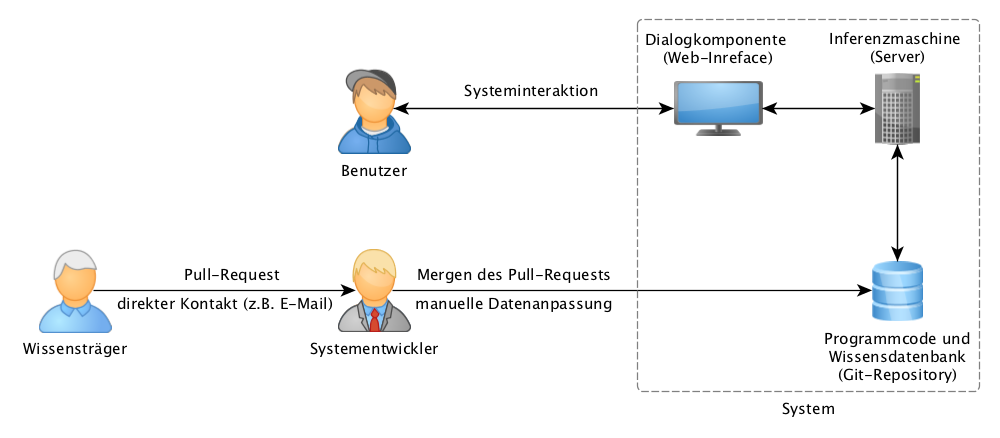
\includegraphics[width=0.9\textwidth]{images/paasfinder.png}
	\caption{Die Struktur von \textit{PaaSfinder}}
	\label{fig:paasfinder}
\end{figure} 
\textit{PaaSfinder} setzt sich aus dem Programmcode der Wissensdatenbank und der Webanwendung zusammen. Die Webanwendung wird wiederum auf einem Server betrieben. Ein Vendor wird in einem Profil\footnote{https://github.com/stefan-kolb/paas-profiles\#profile-specification} beschrieben, das wie folgt aufgebaut ist:
\begin{enumerate}
\item \textbf{General Properties}: allgemeine Eigenschaften des Vendors (z.B.\ Name, \acs{URL} oder \acs{URI}, Status, Typ etc.)
\item \textbf{Extensible}: generelle Erweiterungsm�glichkeit nach Kundenbedarf (z.B.\ spezielle Laufzeitumgebung)
\item \textbf{Pricing}: verf�gbare Preismodelle
\item \textbf{Quality of Service}: die Servicequalit�t (z.B.\ Verf�gbarkeit)
\item \textbf{Hosting}: Art der Bereitstellung (z.B.\ privat)
\item \textbf{Scaling}: Skalierbarkeit (z.B.\ Speichererweiterung)
\item \textbf{Runtimes}: unterst�tzte Laufzeitumgebungen (z.B.\ Java\footnote{https://java.com})
\item \textbf{Middleware} (z.B.\ Tomcat\footnote{https://tomcat.apache.org})
\item \textbf{Frameworks} (z.B.\ Play\footnote{https://www.playframework.com})
\item \textbf{Services} (z.B.\ Datenspeicher)
\item \textbf{Infrastructures} (z.B.\ Informationen zum Standort)
\end{enumerate}
Ein Vendor wird als \acs{JSON}\footnote{\label{foot:json}http://json.org}-Eintrag gespeichert. JSON ist ein Datenaustauschformat und basiert auf zwei Datenstrukturen: 
\begin{itemize}
\item \textit{Name/Wert Paar}, das ein Objekt darstellt (siehe Abbildung \ref{fig:json-object}).
\item \textit{Eine geordnete Liste von Werten (Array)}, die kein oder mehrere durch Komma getrennte Objekte enth�lt (siehe Abbildung \ref{fig:json-array}).
\end{itemize}
\begin{figure}[H] 
	\centering
	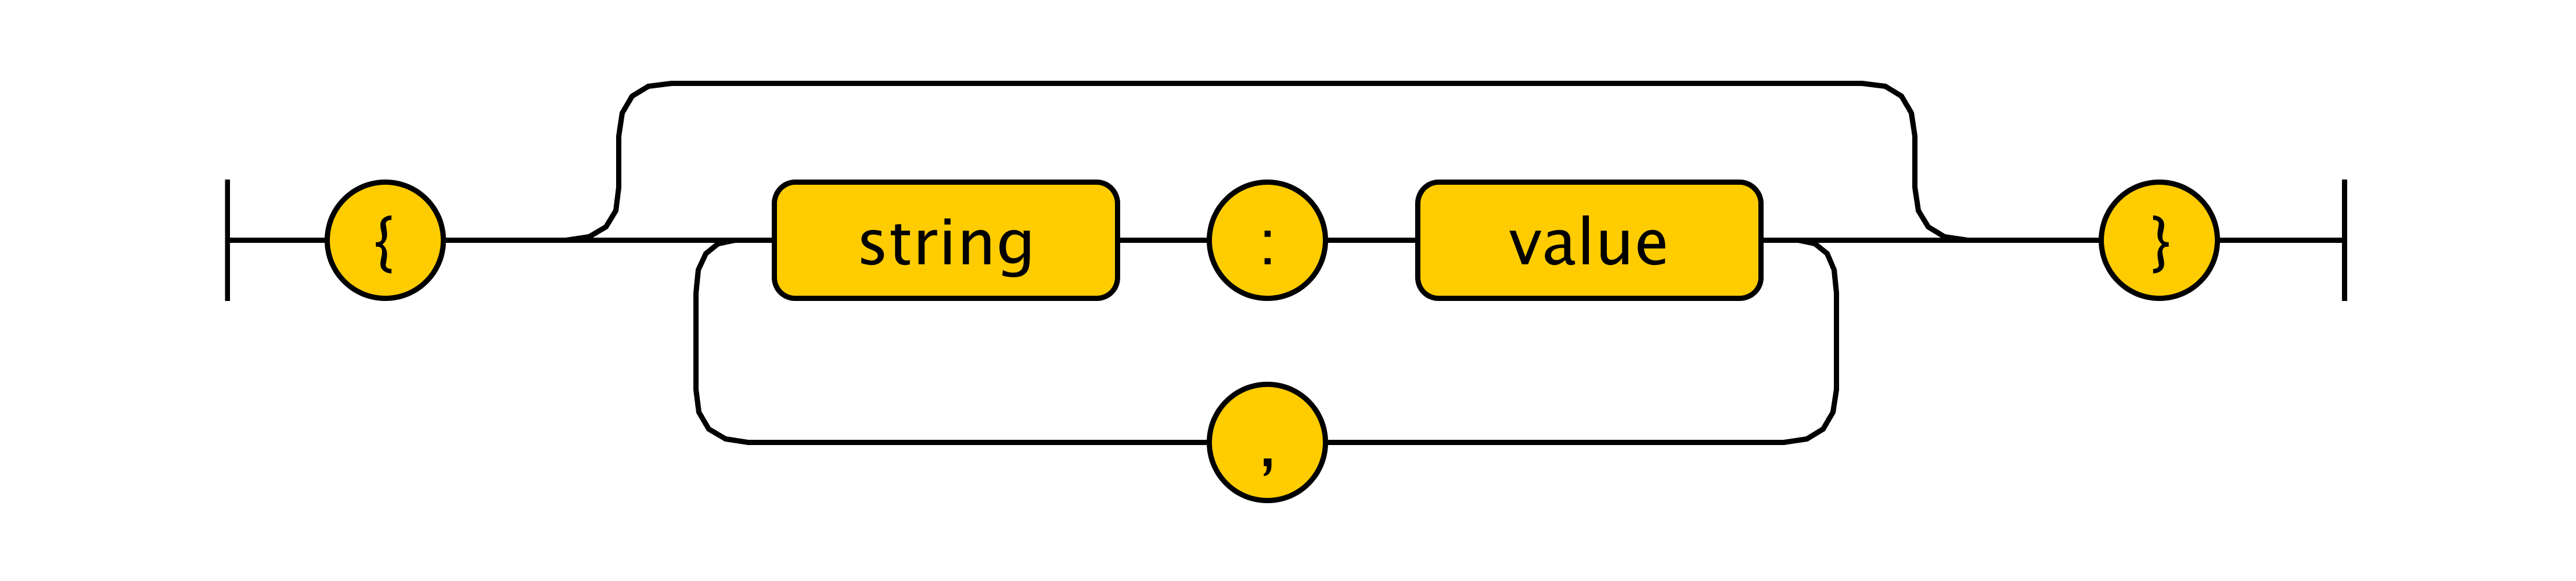
\includegraphics[width=0.85\textwidth]{images/json-object.png}
	\caption{JSON-Objekt Spezifikation}
	\label{fig:json-object}
\end{figure} 
\begin{figure}[H] 
	\centering
	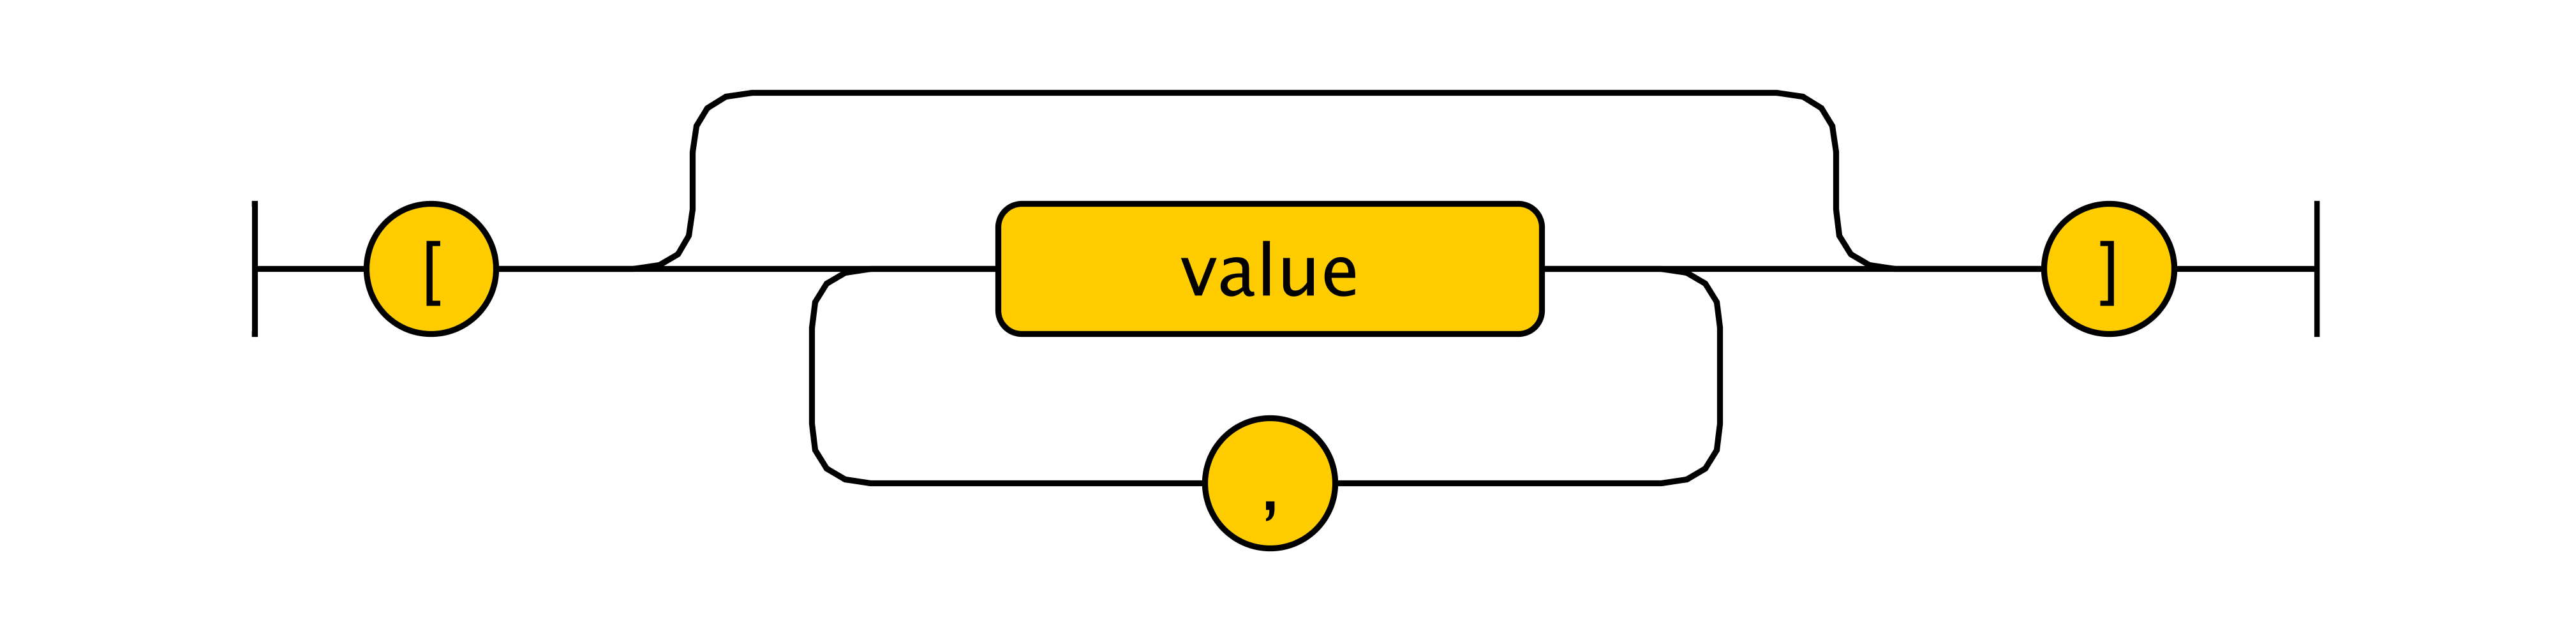
\includegraphics[width=0.75\textwidth]{images/json-array.png}
	\caption{JSON-Array Spezifikation}
	\label{fig:json-array}
\end{figure} 
Die Wissensdatenbank und der Programmcode von \textit{PaaSfinder} befinden sich in einem Git-Repository. Bei Git\footnote{https://git-scm.com} handelt es sich um eine Anwendung zur verteilten Projektverwaltung. Da \textit{PaaSfinder} ein Open-Source-Projekt ist, kann im Prinzip jeder die Wissensdatenbank erweitern bzw. modifizieren. Momentan kann das auf zwei Weisen erfolgen (siehe Abbildung \ref{fig:paasfinder}):
\begin{itemize}
\item \textit{Pull Request\footnote{https://git-scm.com/docs/git-request-pull}}
\item \textit{Direkter Kontakt mit dem Systementwickler} 
\end{itemize}
Beim Pull Request wird zuerst das gesamte Git-Repository lokal gespeichert. Danach werden �nderungen vorgenommen und anschlie�end eine Anfrage beim Projektmaster gestellt. Diese wird vom Projektmaster �berpr�ft und zugeh�rige �nderungen �bernommen (\glqq{}gemerged\grqq{}), falls keine Konflikte mit vorhandenen Daten vorliegen. Wenn der Wissenstr�ger mit dem Git-System nicht vertraut ist, kann direkter Kontakt (beispielsweise per E-Mail) mit dem Systementwickler aufgenommen werden. Die Daten werden dann manuell vom Systemverwalter in die Wissensbasis eingetragen.\\
Sowohl Pull Requests, als auch der Kontakt mit dem Systementwickler entsprechen dem direkten Wissenserwerb gem�� der Klassifikation in Kapitel \ref{subsec:Wissenserwerbskomponente}. Der Vorteil dabei ist, dass die Daten nicht manuell gesucht werden m�ssen, sondern direkt vom Wissenstr�ger stammen. Andererseits wird die Datenerfassung durch fehlende Git-Kenntnisse des Wissenstr�gers beschr�nkt. Um den direkten Wissenserwerb zu erleichtern, wird im weiteren Verlauf die Wissenstr�gerschnittstelle entwickelt, die es dem Wissenstr�ger erm�glicht, einen bestehenden Vendor zu aktualisieren. Nach dem erfolgreichen Absenden der �nderungen soll automatisch ein Pull Request erstellt werden. 
\subsection{Wissenstr�gerschnittstelle}\label{subsec:Wissenstr�gerschnittstelle}
Als erster Schnitt in der Automatisierung der Datenerfassung bei \textit{PaaSfinder} wird eine Schnittstele zur Dateneingabe entwickelt (Wissenstr�gerschnittstelle). Mithilfe der Schnittstelle soll die Aktualisierung eines bestehenden Profils erm�glicht werden. Das Anlegen oder das L�schen eines Profils liegt nicht im Anwendungsbereich der Schnittstelle. Der Ablauf wird in Abbildung \ref{fig:update-allgemein} veranschaulicht.
\begin{figure}[H] 
	\centering
	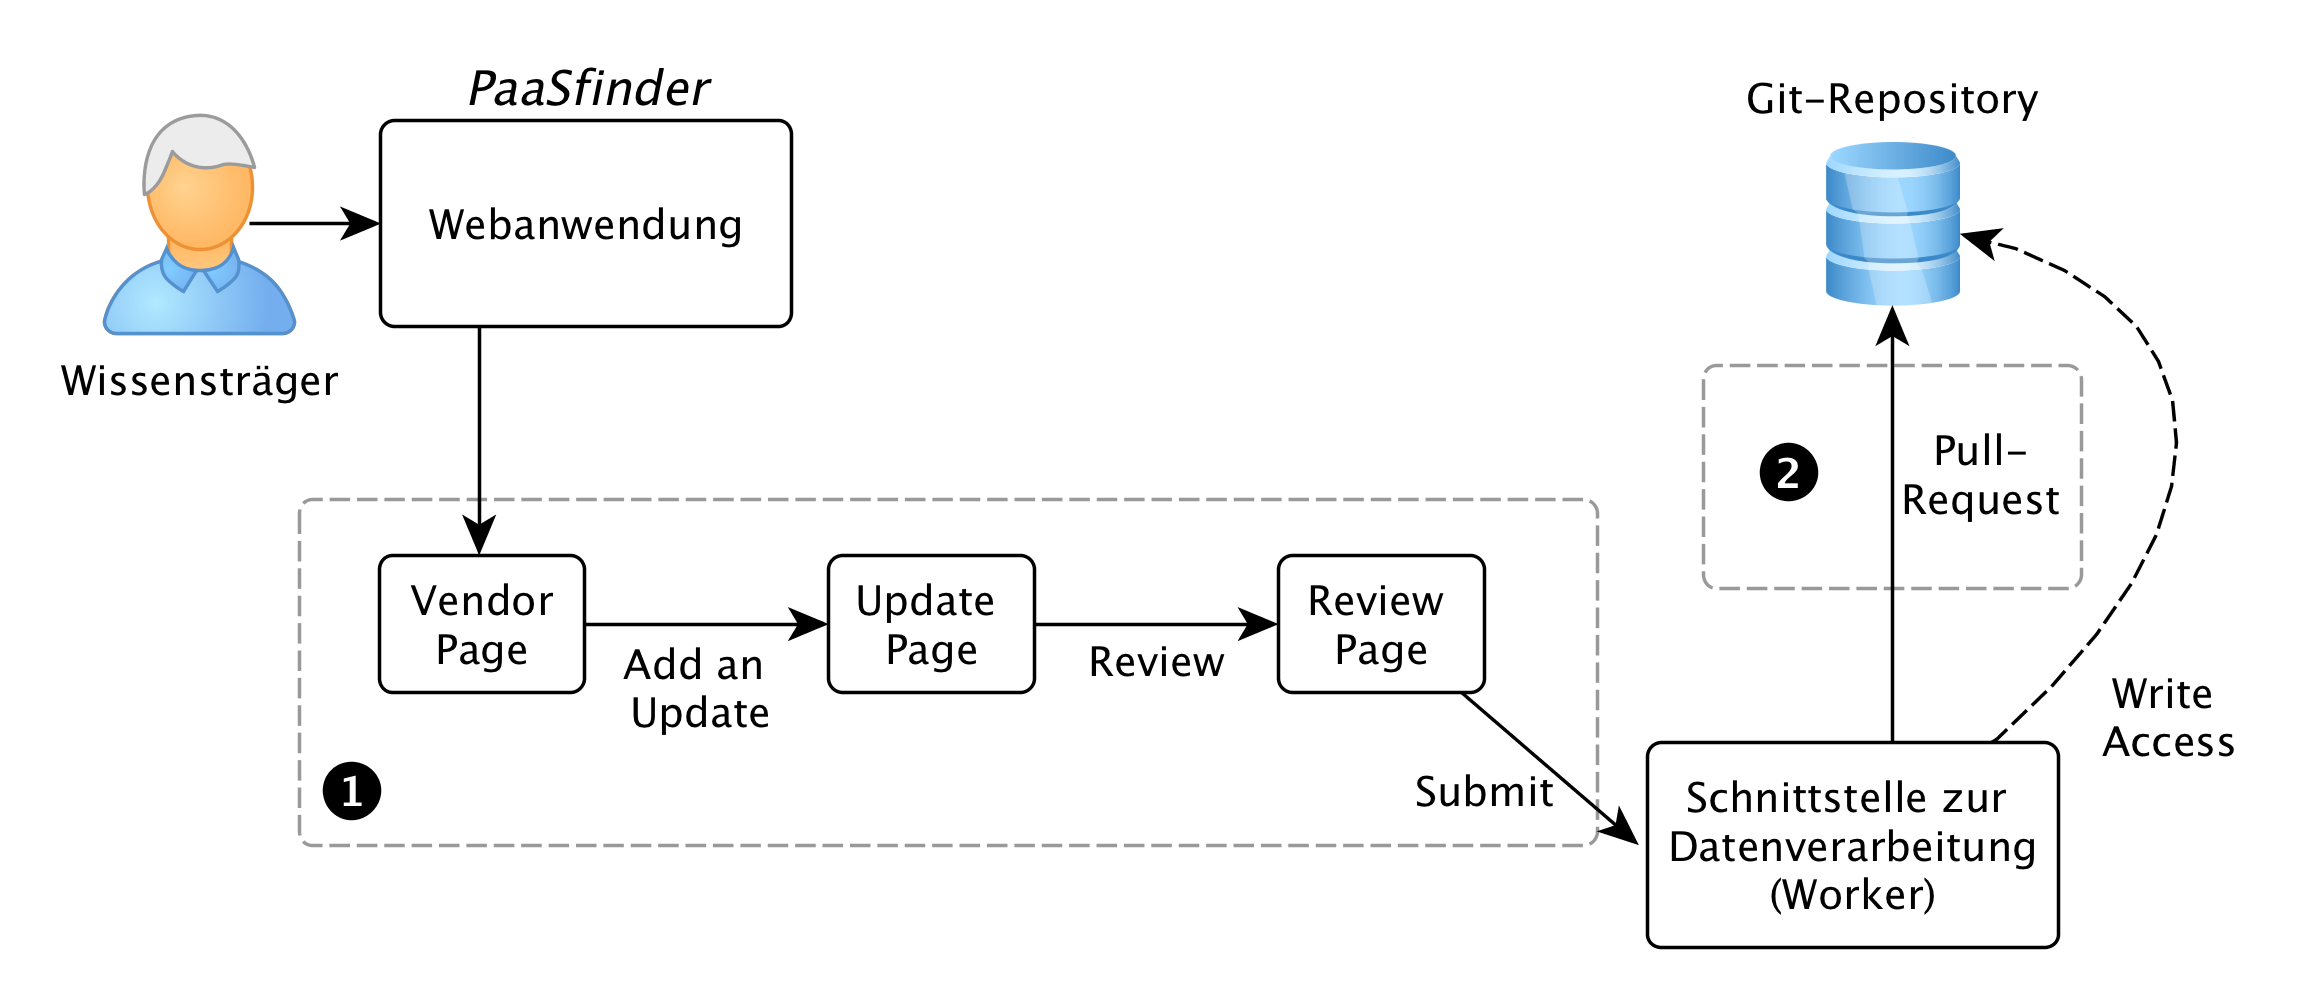
\includegraphics[width=1.0\textwidth]{images/update.png}
	\caption{Profilaktualisierung mittels Wissenstr�gerschnittstelle}
	\label{fig:update-allgemein}
\end{figure}
Der Ablauf in Abbildung \ref{fig:update-allgemein} l�sst sich in zwei Schritte aufteilen. Dieser Abschnitt besch�ftigt sich mit dem ersten Schritt, der die Daten von einem Wissenstr�ger entgegennimmt, zusammenfasst und abschickt. Die Verarbeitung dieser Daten erfolgt im zweiten Schritt, der im n�chsten Abschnitt besprochen wird. Allgemein besteht der erste Schritt aus folgenden Aktionen:
\begin{enumerate}
\item \textit{Profilauswahl} (Vendor Page)
\item \textit{Aktualisieren} des Profils (Update Page)
\item \textit{�berpr�fung} der Daten (Review Page)
\item \textit{Absenden} der Daten (Sumbit)
\end{enumerate}
Der gesamte Prozess l�sst sich in Abbildung \ref{fig:activity} als ein Aktivit�tsdiagramm darstellen. Die verwendete Notation entspricht dem UML-Standard 2.5 \footnote{http://www.omg.org/spec/UML/2.5/PDF}. Es werden Knoten (Rechteck) f�r Aktivit�ten und Kanten (Pfeile) f�r Verbindungen verwendet. Bei den Verbindungen werden Kontrollfluss- und Datenflussverbindungen unterschieden. Im Fall einer Datenflussverbindung gibt es ein Ein- und der Ausgabe-Pin (kleiner Quadrat) am Anfang oder am Ende des Pfeils. Im vorliegenden Fall werden noch Fallunterscheidungen verwendet, die durch eine Raute gekennzeichnet sind.
\begin{figure}[H] 
	\centering
	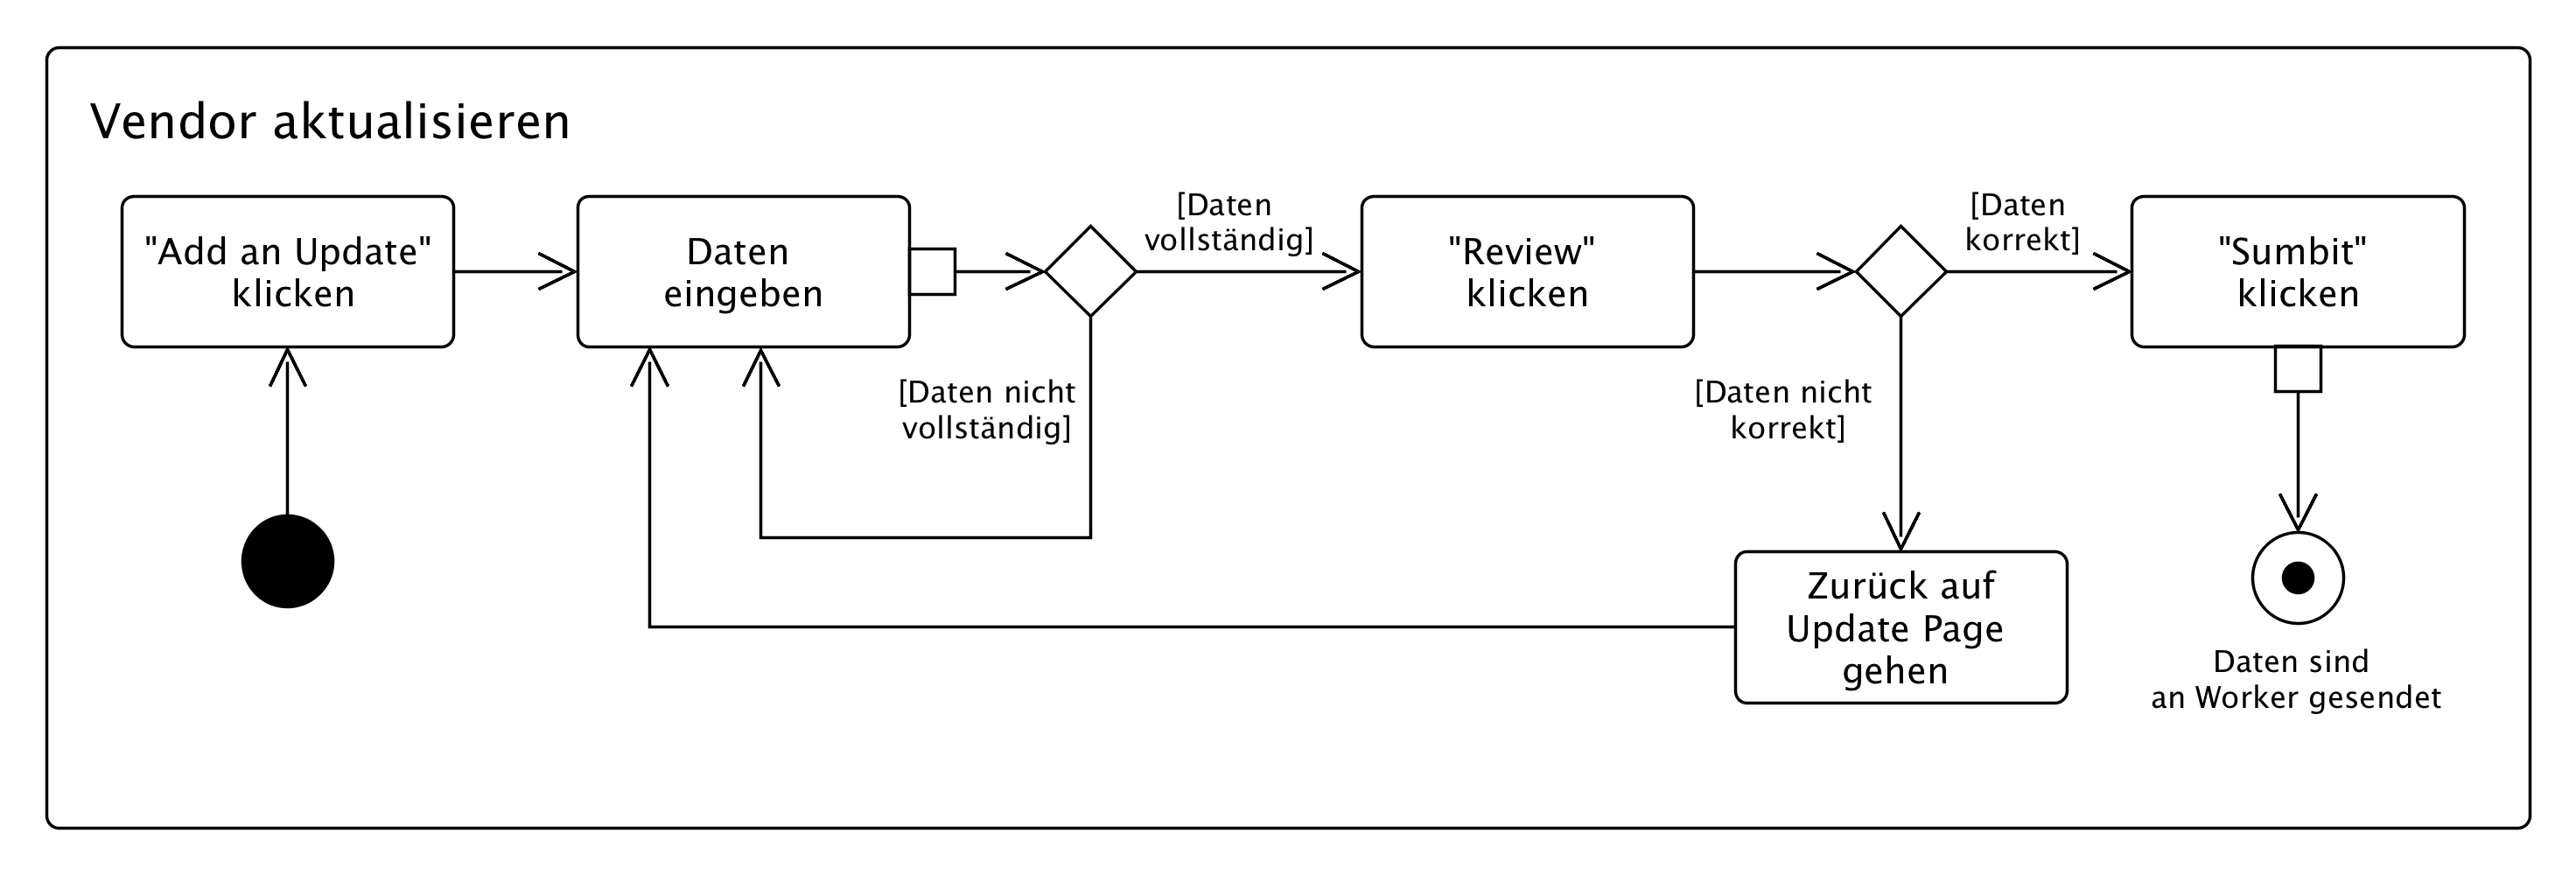
\includegraphics[width=1.0\textwidth]{images/activity.png}
	\caption{Aktivit�tsdiagramm der Aktualisierung des PaaS-Profils}
	\label{fig:activity}
\end{figure}
Ausgehend von einer Vendor Page wird der Ablauf mit \glqq{}Add an Update\grqq{} gestartet. Als n�chstes werden die Daten eingegeben. Wenn das Profil aus Sicht des Wissenstr�gers vollst�ndig ist, wird auf \glqq{}Review\grqq{} geklickt. Sonst wird der Schritt der Dateneingabe wiederholt. Falls der \glqq{}Review\grqq{}-Button geklickt wurde, gelangt man zur Review Page. Hier k�nnen die Daten �berpr�ft werden. Wenn die Daten korrekt sind, kann das aktualisierte Profil mit dem Klick auf \glqq{}Submit\grqq{} an den Worker gesendet werden. Anderenfalls kann der Wissenstr�ger zur�ck zur Dateneingabe gehen und die Daten �berarbeiten. In jedem Zeitpunkt besteht die M�glichkeit, den Vorgang abzubrechen, indem das Browserfenster geschlossen wird. Die Daten werden nur dann gesendet, wenn der \glqq{}Submit\grqq{}-Button auf der Review Page geklickt wird. Im weiteren Verlauf wird die Implementierung der Page und Review Page beschrieben.\\
Die Update Page umfasst zwei Aspekte. Erstens sollen die Profildaten f�r den Wissenstr�ger geeignet dargestellt werden Zweitens soll die Eingabe der Daten erm�glicht werden. Au�erdem sollen die �nderungen am Profil dynamisch zwischengespeichert werden. Das ist eine herausfordernde Aufgabe, da ein Profil, abgesehen von allgemeinen Eigenschaften (z.B. \glqq{}name\grqq{}), aus komplexen und teils verschachtelten Datentypen besteht. In Abbildung \ref{fig:profil} wird das am Beispiel von \glqq{}runtimes\grqq{} (Laufzeitumgehungen) gezeigt. Farbe gelb steht dabei f�r ein Objekt, grau f�r eine Liste und wei� f�r ein String (Zeichenkette). Hier umfasst ein Profil (\glqq{}vendor\grqq{}) eine Liste von \glqq{}runtimes\grqq{}. \glqq{}Runtime\grqq{} besteht wiederum aus \glqq{}language\grqq{} und \glqq{}versions\grqq{}.
\begin{figure}[H] 
	\centering
	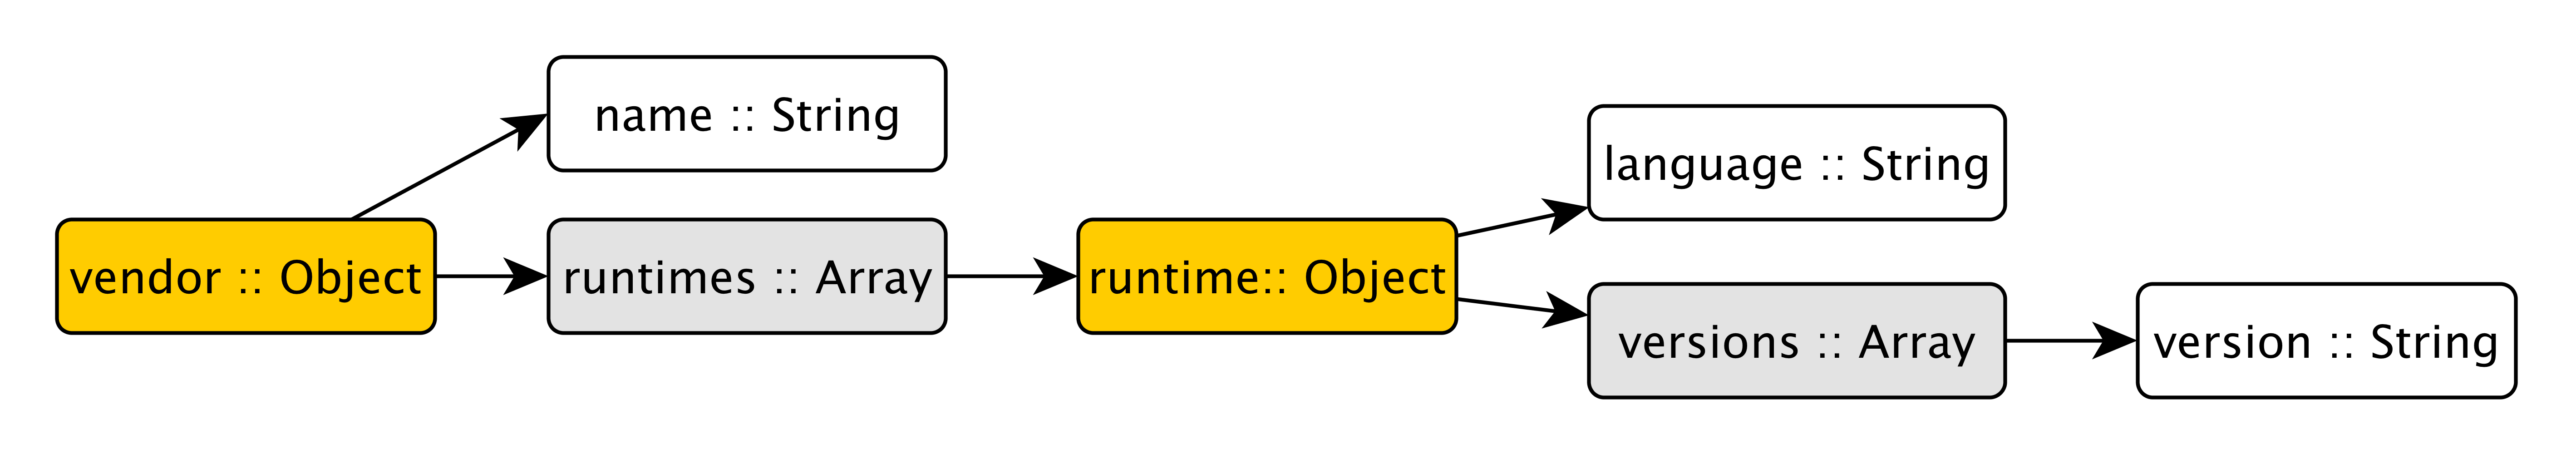
\includegraphics[width=0.90\textwidth]{images/vendor.png}
	\caption{Komplexe Datentypen im PaaS-Profil}
	\label{fig:profil}
\end{figure}
Um diese Aufgabe zu l�sen, werden die Daten in zwei Richtungen gebunden (two-way data binding). Zu diesem Zweck wird ein Open-Source Framework Knockout.js\footnote{http://knockoutjs.com} eingesetzt. Knockout.js ist eine JavaScript Bibliothek zur Erstellung dynamischer Webseiten. Das Framework basiert auf \ac{MVVM} Entwurfsmuster\footnote{http://knockoutjs.com/documentation/observables.html}:
\begin{itemize}
\item \textit{Model}: Daten, die unabh�ngig auf einem Server liegen (hier: verf�gbare PaaS-Profile)
\item \textit{ViewModel}: Programmcode der Daten und Operationen auf der Benutzerschnittstelle (hier: JavaScript Klasse f�r PaaS-Profil (Modell))
\item \textit{View}: Benutzerschnittstelle, die den Zustand von ViewModel abbildet und bei Benutzeraktionen aktualisiert (hier: Update Page)
\end{itemize}
Als erstes werden die f�r das Modell erforderliche Daten �ber \textit{PaaSfinder}-\acs{API}\footnote{https://paasfinder.org/api/vendors/} geholt und das Modell initialisiert. Da das Modell komplexe Datentypen umfasst, sind explizite JavaScript Klassen n�tig. Beispielsweise gibt es f�r \glqq{}runtime\grqq{} und \glqq{}version\grqq{} jeweils eigene Klassen mit unterschiedlichem Verhalten. Die Klasse \glqq{}runtime\grqq{} beinhaltet z.B. die Methode zum Hinzuf�gen neuer Version. Nachdem das Modell initialisiert wurde, wird das Data-Binding zwischen dem Modell und der View aktiviert.\\
W�hrend die Update Page die Benutzerdaten entgegennimmt, werden die Daten auf der Review Page zusammenfasst, so dass der Wissenstr�ger die Eingaben �berpr�fen kann. Die Profildaten von der Update zur Review Page werden mithilfe von Web Storage\footnote{https://www.w3.org/TR/webstorage/} ausgetauscht. W3C definiert zwei Arten der Speicherung, n�mlich Session und Local Storage. Session Storage gilt ausschlie�lich innerhalb Browserfenster. Die Inhalte von Local Storage k�nnen dagegen innerhalb einer Domain zugegriffen werden und gelten zeitlich unbeschr�nkt. Selbst beim Fensterschlie�en bleiben die Daten erhalten und k�nnen bei Bedarf gelesen werden. Daher wird im Weiteren Local Storage betrachtet.\\
Auf der Update Page wird das Profil beim Klicken auf \glqq{}Review\grqq{} in die Local Storage gespeichert. Das Speichern bzw. Lesen basiert wie bei JSON auf Schl�ssel/Wert-Paar-Prinzip. Der Schl�ssel ist dabei der Profilname, der bei der API benutzt wird. Da der Schl�ssel als Parameter an die Review Page geschickt wird, k�nnen die Daten problemlos gelesen werden. Es besteht ebenso die M�glichkeit, das Profil auf der Update Page zur�ckzusetzen, indem die Profildaten aus der Local Storage gel�scht und erneut von der \textit{PaaSfinder}-API angefordert werden.\\
Im folgenden Beispiel wird das Profil \glqq{}Heroku\grqq{} aktualisiert, indem eine neue Version (1.9) zu Java in \glqq{}runtimes\grqq{} hinzugef�gt wird.
\begin{enumerate}
\item Von der Vendor Page auf \glqq{}Add an Update\grqq{} klicken.
	\begin{figure}[H] 
		\centering
		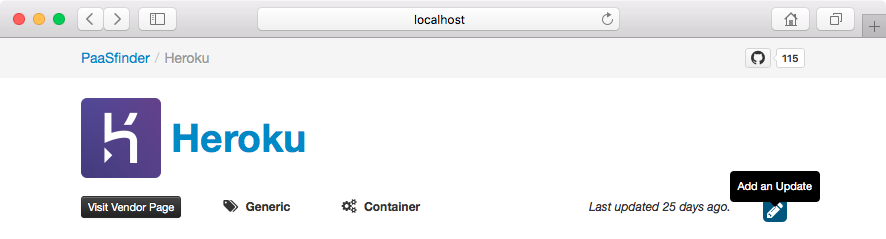
\includegraphics[width=1.0\textwidth]{images/ablauf/vendor-page.png}
		\caption{Vendor Page}
		\label{fig:vendor-page}
	\end{figure}
\item Eine neue Java Version (1.9) hinzuf�gen (siehe Abbildung \ref{fig:update-page}).
	\begin{figure}[H] 
		\centering
		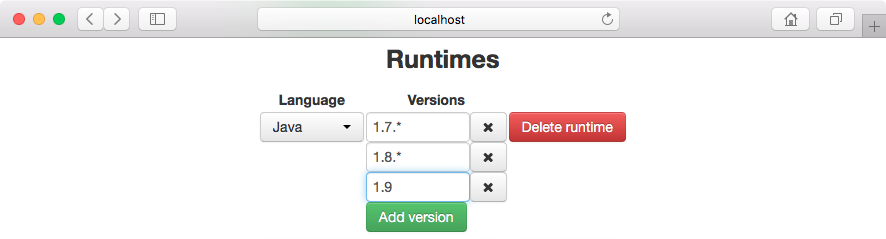
\includegraphics[width=1.0\textwidth]{images/ablauf/update-page.png}
		\caption{Update Page}
		\label{fig:update-page}
	\end{figure} 
\item Die Daten auf der Review Page �berpr�fen (siehe Abbildung \ref{fig:vendor-page}).
	\begin{figure}[H] 
		\centering
		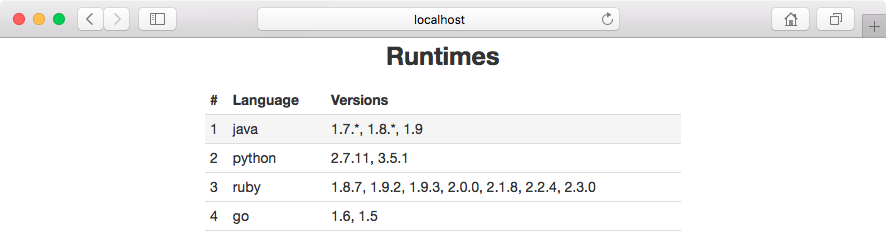
\includegraphics[width=1.0\textwidth]{images/ablauf/review-page.png}
		\caption{Review Page}
		\label{fig:review-page}
	\end{figure} 
\item Optional kann der Wissenstr�ger seine Kontaktdaten (Name und E-Mail) sowie die Nachricht zum Update hinterlassen.
	\begin{figure}[H] 
		\centering
		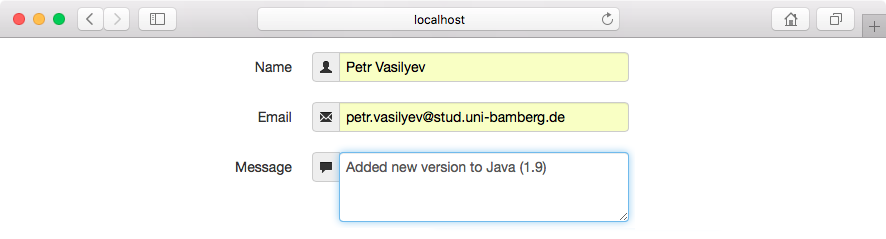
\includegraphics[width=1.0\textwidth]{images/ablauf/kontaktform.png}
		\caption{Kontaktdatenform}
		\label{fig:kontaktdatenform}
	\end{figure} 
\item Anschlie�end werden die Daten mit dem Klick auf den \glqq{}Sumbit\grqq{}-Button an die f�r die Daten�bermittlung zust�ndige Schnittstelle abgeschickt.
\end{enumerate}
Ein wichtiger Aspekt bei der Entwicklung der Wissenstr�gerschnittstelle ist die Validierung der Eingabedaten. In einigen F�llen k�nnen problematische Eingaben bereits auf der Ebene der Benutzerschnittstelle (User Interface) verhindert werden. Als Beispiel wird in der Kontaktform (Abbildung \ref{fig:kontaktdatenform}) bei der E-Mail Adresse mittels HTML-Attributes type=\glqq{}email\grqq{} sichergestellt, dass der Input formal der E-Mail Struktur einspricht. Allerdings kann der vergleichbare Ansatz nicht immer angewandt werden. Ein Beispiel ist eine Version, die ein Sonderzeichen (z.B. *) oder einen Buchstaben enthalten kann.
\subsection{Worker f�r Daten�bermittlung}\label{subsec:Worker}
Der vorliegende Abschnitt befasst sich mit dem Teil der Wissenserwerbskomponente, der als Bindeglied zwischen den Wissenserfassungsmethoden und der Wissensbasis auftritt und in Abbildung \ref{fig:wissenserwerbskomponente} als Schnittstelle f�r die Daten�bermittlung bezeichnet wird. Im Rahmen dieser Arbeit wird der Begriff \glqq{}\textit{Worker}\grqq{} verwendet, der f�r die Auspr�gung dieser Schnittstelle steht. Im Folgenden wird das Konzept hinter dem Worker abstrakt skizziert und im weiteren Verlauf mit der konkreten Implementierung verdeutlicht. Der Anwendungsbereich des Workers wird in Abbildung \ref{fig:worker} wie folgt dargestellt:
\begin{figure}[H] 
	\centering
	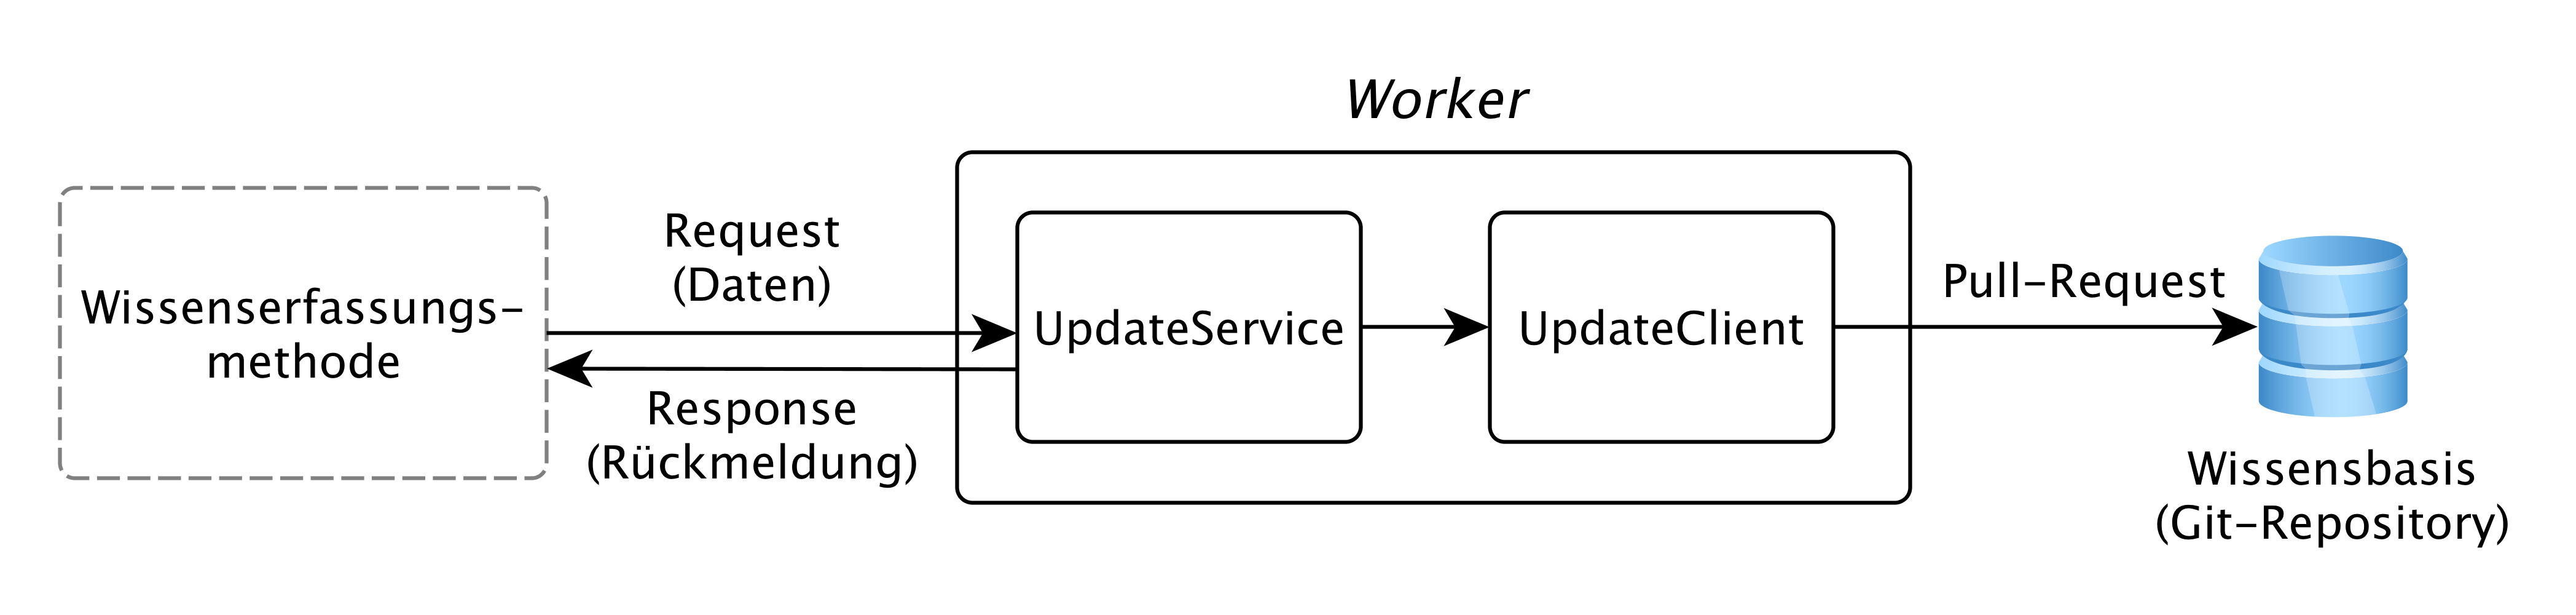
\includegraphics[width=1.0\textwidth]{images/anwendungsbereich_worker.png}
	\caption{Anwendungsbereich vom Worker}
	\label{fig:worker}
\end{figure}
Grunds�tzlich besteht der Worker aus zwei Komponenten, n�mlich \glqq{}\textit{UpdateService}\grqq{} und \glqq{}\textit{UpdateClient}\grqq{}. Die Aufgabe des UpdateService besteht in der Bereitstellung einer Schnittstelle, die die Daten von au�en aufnimmt und die Daten�bermittlung an den UpdateClient delegiert. Auf der anderen Seite stellt der UpdateClient die Methoden zur Verf�gung, die f�r die Daten�bermittlung zust�ndig sind.\\
Generell l�sst sich der Ablauf gem�� Abbildung \ref{fig:worker} folgenderma�en beschreiben. Als erstes werden die Daten von der Wissenserfassungsmethode an den UpdateService gesendet. Darauffolgend werden die Daten vom UpdateService verarbeitet und f�r den UpdateClient vorbereitet. Im n�chsten Schritt wird die Aufgabe der Daten�bermittlung an den UpdateClient delegiert. Der UpdateClient erstellt die Anfrage an die Wissensbasis und teilt die Antwort dem UpdateService mit. Anschlie�end verschickt der UpdateService die R�ckmeldung an die Wissenserfassungsmethode.\\ 
Des Weiteren wird die Wissenstr�gerschnittstelle aus dem Abschnitt \ref{subsec:Wissenstr�gerschnittstelle} als Wissenserfassungsmethode betrachtet. Die Wissensbasis stellt das Git-Repository von \textit{PaaSfinder} dar, das von einem Bot-Account auf Github \glqq{}geforkt\grqq{} wird\footnote{https://github.com/update-bot/paas-profiles}. In anderen Worten wird das urspr�ngliche Git-Repository von \textit{PaaSfinder} kopiert, sodass der Bot-Account einen schreibenden Zugriff auf die Wissensbasis erh�lt.\\
Technisch gesehen erfolgt der Nachrichtenaustausch zwischen Wissenserfassungsmethode, dem Worker und der Wissensbasis auf Basis des Hypertext Transfer Protocols (\acs{HTTP}) und des \ac{REST} Prinzips, das urspr�nglich aus der Dissertation von Fielding \cite{fielding2000} stammt. Das zentrale Konzept von REST basiert auf Ressourcen, die im globalen Raum mithilfe eines \ac{URI}\footnote{https://tools.ietf.org/html/rfc3986} eindeutig identifiziert werden \cite[S.11,35]{tilkov2015}. Ein Vendor wird also als Ressource im JSON Format zun�chst zum Worker und anschlie�end zum Git-Repository geschickt.\\
Um die Daten von au�en empfangen zu k�nnen, implementiert der UpdateClient eine REST API, die in Form einer Route (\glqq{}/vendor\grqq{}) definiert wird. Die Route entspricht dem HTTP-Standardverb POST\footnote{https://tools.ietf.org/html/rfc7231\#section-4.3.3} und akzeptiert die Daten im JSON Format. F�r die Implementierung der Route wurde das Framework Spark\footnote{http://sparkjava.com} verwendet. Auf der Seite vom UpdateClient werden die Nachrichten als Anfragen an die Github API\footnote{https://developer.github.com/v3} mithilfe von OkHttp\footnote{https://square.github.io/okhttp}  gesendet. In Java Pseudocode l�sst sich die Route folgenderma�en beschreiben (siehe Listing \ref{service}):
\begin{lstlisting}[basicstyle=\ttfamily, label=service,
					captionpos=b, caption={\glqq{}/vendor\grqq{} Route}]
post("/vendor", "application/json", (request, response) -> {
  JsonObject data = jsonParser.parse(request.body());
  
  Branch branch = new Branch(..);       
  client.postBranch(branch);
  
  File file = new File(..);
  client.putFile(file);

  PullRequest pullRequest = new PullRequest(..);
  client.postPullRequest(pullRequest);
});
\end{lstlisting}
Als erstes werden die Daten in ein Java Objekt transformiert. Danach wird ein neuer Branch erzeugt und an den UpdateClient zum Absenden weitergegeben. Sobald der Branch auf der Github-Seite erfolgreich erstellt wurde, wird die Vendor-Datei im erstellten Branch aktualisiert. Anschlie�end wird ein Pull-Request erzeugt und vom UpdateClient an das Git-Repository geschickt. Bedauerlicherweise l�sst sich der Ablauf nicht parallelisieren, da der n�chste Schritt die erfolgreiche Ausf�hrung des vorherigen Schrittes voraussetzt. Beispielsweise setzt die Aktualisierung der Datei die Erstellung des Branches voraus, da die Datei im erstellten Branch aktualisiert wird.\\ 
Wenn man den oben beschriebenen Ablauf auf das Beispiel mit \glqq{}Heroku\grqq{} aus dem Abschnitt \ref{subsec:Wissenstr�gerschnittstelle} �bertr�gt, ergibt sich Folgendes: sobald der Benutzer auf \glqq{}Submit\grqq{} klickt, werden die Daten als JSON in der POST-Anfrage an den Worker gesendet, n�mlich an die Schnittstelle des UpdateService. Das erfolgreiche Branch- bzw. Pull-Request-Erstellen wird durch den HTTP-Code 201 (\glqq{}Created\grqq{}) im Response der Github-API mitgeteilt (siehe Listing \ref{branch} und \ref{pullrequest}). Beim erfolgreichen Updaten der Datei wird der Statuscode 200 (\glqq{}OK\grqq{}) zur�ckgeliefert (siehe Listing \ref{file}).
\begin{lstlisting}[basicstyle=\ttfamily, breaklines=true, label=branch,
					captionpos=b, caption={Response beim erfolgreichen Branch-Erstellen}]
  protocol=http/1.1,
  code=201, 
  message=Created,
  url=https://api.github.com/repos/update-bot/paas-profiles/git/refs
\end{lstlisting}

\begin{lstlisting}[basicstyle=\ttfamily, breaklines=true, label=file,
					captionpos=b, caption={Response beim erfolgreichen File-Update}]
  protocol=http/1.1,
  code=200, 
  message=OK, 
  url=https://api.github.com/repos/update-bot/paas-profiles/contents/profiles/heroku.json
\end{lstlisting}

\begin{lstlisting}[basicstyle=\ttfamily, breaklines=true, label=pullrequest,
					captionpos=b, caption={Response beim erfolgreichen Pull-Request-Erstellen}]
  protocol=http/1.1,
  code=201,
  message=Created,
  url=https://api.github.com/repos/update-bot/paas-profiles/pulls
\end{lstlisting}
Nach der erfolgreichen Pull-Request-Erstellung kann die aktualisierte Version von Heroku auf Github angeschaut werden (siehe Abbildung \ref{fig:pull-requests}). In der Detailansicht werden ebenso die �nderungen explizit gezeigt. Dabei werden die gel�schten Zeilen als rot markiert und die hinzugef�gten als gr�n (siehe Abbildung \ref{fig:pull-request-detail}).
\begin{figure}[H] 
	\centering
	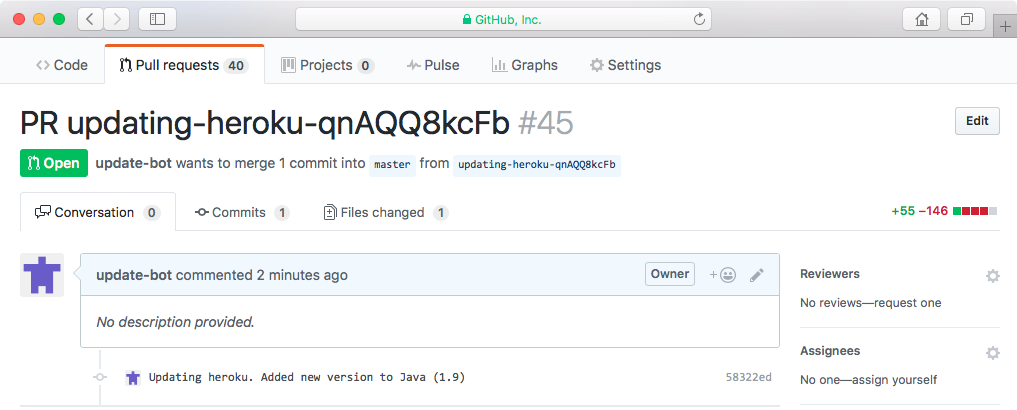
\includegraphics[width=1.0\textwidth]{images/pull-requests.png}
	\caption{Pull-Requests Ansicht auf Github}
	\label{fig:pull-requests}
\end{figure}
\begin{figure}[H] 
	\centering
	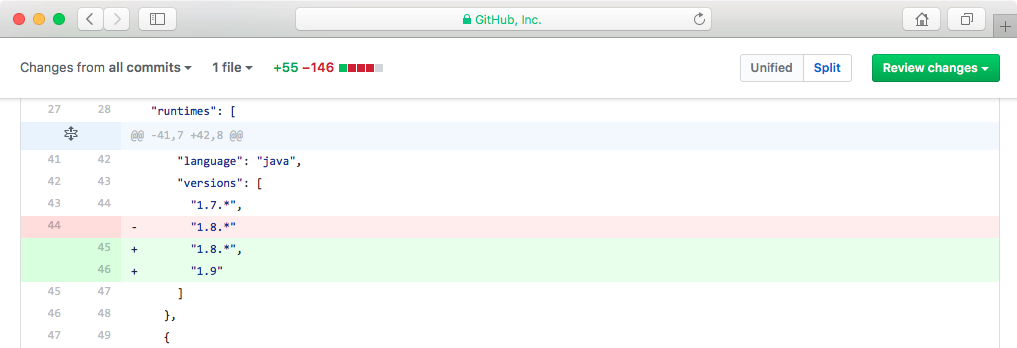
\includegraphics[width=1.0\textwidth]{images/pull-request-detail.png}
	\caption{Heroku Pull Request}
	\label{fig:pull-request-detail}
\end{figure}
Schlie�lich wird im Erfolgsfall der Statuscode 200 (\glqq{}OK\grqq{}) der Wissenserfassungsmethode mitgeteilt. In Bezug auf die Fehlerbehandlung wird jeder Schritt, der sich logisch abgrenzen l�sst (Branch erstellen, Datei aktualisieren und Pull-Request erstellen), in einem eigenen try-catch-Block innerhalb der Route in Listing \ref{service} ausgef�hrt, sodass der Client eine aussagekr�ftige Fehlermeldung erh�lt.
\newpage
\section{Ausblick}\label{sec:Ausblick}
Nachdem die Wissenstr�gerschnittstelle zur Datenkorrektur und der Worker zum Erstellen automatischer Pull Requests betrachtet wurden, handelt es sich im vorliegenden Abschnitt um einen Ausblick auf weitere Datenquellen, die ein Automatisierungspotential im Rahmen der Datenerfassung f�r \textit{PaaSfinder} aufweisen. Nach einer kurzen Erl�uterung der m�glichen Datenquellen findet ein Vergleich der Quellen statt. Anschlie�end wird ein Bezug auf zuk�nftige Arbeiten genommen. 
\subsection{Abgrenzung der Datenquellen}\label{subsec:Abgrenzung der Datenquellen}
Die Auswahl der Datenquellen erfolgt unter der Annahme, dass die Datenerfassung sich auf die Aktualisierung der bestehenden Vendors beschr�nkt. Der Grund daf�r besteht darin, dass die maschinelle Erfassung eines neuen Vendors die fachliche Expertise eines Experten erfordert. \\
Insgesamt k�nnen folgende Datenquellen relevant sein:
\begin{itemize}
\item Webseite des Vendors
\item Web-Feeds
\item Soziale Netzwerke 
\item Newsletter
\item Blogs
\end{itemize}
Die erste Quelle, die bei der Datenerfassung eines Vendors in Frage kommt, ist dessen Web\-auf\-tritt. Zur Datenerfassung kann ein Web-Crawler benutzt werden, der ausgehend von einem Startlink (Seed) und nach einem Suchbegriff die Webseite durchsucht \cite[S.32]{croft2010}. Als Seed wird die Homepage des Vendors verwendet. Die weiteren Seiten ergeben sich durch Verfolgen der Links auf der besuchen Seite. Allerdings ist dieser Ansatz hier weniger sinnvoll, da die Mehrheit der Daten in \textit{PaaSfinder} bereits vorliegt.\\
Bei Web-Feeds handelt es sich um \glqq{}Content Syndication\grqq{}, was als Bereitstellung von Daten f�r �bertragung, Aggregierung und Online-Publikation\footnote{http://web.resource.org/rss/1.0/} bezeichnet werden kann. Ein verbreitetes Beispiel f�r Web-Feeds ist RSS. Die Abk�rzung steht je nach Quelle f�r \glqq{}RDF Site Summary\grqq{}\footnote{http://web.resource.org/rss/1.0/spec}, \glqq{}Really Simple Syndikation\grqq{}\footnote{https://validator.w3.org/feed/docs/rss2.html} oder \glqq{}Rich Site Summary\grqq{}. Es wird zwischen Push und Pull RSS unterschieden. Bei Push RSS werden die Benachrichtigung vom Absender angesto�en. Bei Pull RSS soll der Nutzer die Benachrichtigungen manuell abrufen. In der Praxis werden Pull RSS am meisten eingesetzt. Ein RSS-Dokument wird in XML-Format beschrieben, was ein effizientes Parsen der Inhalte erm�glicht. Au�erdem enthalten RSS-Eintr�ge das Erstellungsdatum, das f�r die Zuordnung der Aktualisierung hilfreich ist. Ein RSS Beispiel von Heroku\footnote{https://www.heroku.com/} wird in Listing \ref{rss} dargestellt.
\begin{lstlisting}[basicstyle=\ttfamily, breaklines=true, label=rss,
					captionpos=b, caption={Ein RSS-Beispiel von Heroku}]
<rss xmlns:dc="http://purl.org/dc/elements/1.1/" version="2.0">
 <channel>
  <title>Heroku</title>
  <link>http://blog.heroku.com</link>
  <description>The Heroku Blog</description>
  <item>
   <title>The Heroku-16 Stack is Now Available</title>
   <link>https://blog.heroku.com/heroku-16-is-generally-available</link>
   <pubDate>Thu, 20 Apr 2017 15:06:00 GMT</pubDate>
   <guid>https://blog.heroku.com/heroku-16-is-generally-available</guid>
   <description>
    <p>Your Heroku applications run on top of ...</p> 
   </description>
   <author>Jon Byrum</author>
  </item>
 </channel>
</rss>
\end{lstlisting}
Neben RSS k�nnen soziale Netzwerke f�r das Beziehen von Updates verwendet werden. Twitter\footnote{https://twitter.com/} ist ein Beispiel daf�r. Der Vorteil dieses Kurznachrichtendienstes besteht darin, dass er f�r den Vendor keinen Entwicklungsaufwand mitbringt. Zum Abrufen der Daten bietet Twitter eine eigene REST API\footnote{https://dev.twitter.com/rest/public} an.\\
Newsletter und Blogs k�nnen ebenso als potentielle Datenquellen benutzt werden. Beim Abonnieren von Newslettern werden vom Vendor regelm��ig die Updates an die E-Mail Adresse verschickt. Au�erdem k�nnen Vendor Blogs zur Datenerfassung durchsucht werden. In einem Blog werden meist Informationen ver�ffentlicht, die f�r Entwickler interessant sind. Ein Blogeintrag ist meist ein kurzer Artikel, der ein Update enth�lt. Aus diesem Grund werden Blogs ebenso f�r die Datenerfassung in Betracht gezogen.
\subsection{Vergleich der Informationsquellen}\label{subsec:vergleich}
Im Zuge des Vergleich wurden 30 Vendors (n=30) nach Vorhandensein der Informationsquellen ausgewertet. Als Informationsquellen wurden RSS-Feeds, Twitter und Newsletter ausgew�hlt. Ein weiteres Kriterium in der Auswertung ist das Datum des letzten Updates. Das Datum wird nach dem neuesten Eintrag zwischen den vorliegenden Informationsquellen zum Zeitpunkt 10.05.2017 bestimmt. Die Zusammenfassung der Ergebnisse wird in Tabelle \ref{tab:vergleich} dargestellt: 
\begin{table}[H] 
\centering 
\begin{tabular}{ |l|c|c|c|c| }
\hline
\textbf{Vendor} & \textbf{RSS} & \textbf{Twitter} & \textbf{Newsletter} & \textbf{Last Update} \\ \hline
\hline
Anynines & nein & ja & ja & 18.08.15 \\ \hline
App42 PaaS & nein & ja & nein & 10.05.17 \\ \hline
AppFog & nein & ja & ja & 10.05.17 \\ \hline
AppHarbor & nein & ja & nein & 22.05.16 \\ \hline
BitNami & nein & ja & nein & 10.05.17 \\ \hline
Brightbox & nein & ja & nein & 25.04.17 \\ \hline
Clever Cloud & nein & ja & nein & 26.04.17 \\ \hline
Cloudnode & nein & ja & nein & 23.04.17 \\ \hline
CloudUnit & nein & ja & nein & 10.05.17 \\ \hline
Cloudways & nein & ja & ja & 10.05.17 \\ \hline
EngineYard & nein & ja & nein & 29.04.17 \\ \hline
Flynn & nein & ja & ja & 17.10.16 \\ \hline 
fortrabbit & nein & ja & nein & 04.05.17 \\ \hline
Getup Cloud & nein & ja & nein & 09.05.17 \\ \hline
Google App Engine & nein & ja & ja & 10.05.17 \\ \hline
Heroku & ja & ja & ja & 10.05.17 \\ \hline
Jelastic & nein & ja & ja & 10.05.17 \\ \hline
Mendix & nein & ja & nein & 28.04.17 \\ \hline
mOSAIC & ja & nein & nein & 05.04.13 \\ \hline
OpenShift Container Platform & nein & ja & nein & 22.04.17 \\ \hline
Oracle Cloud PaaS & ja & ja & nein & 01.12.16 \\ \hline
OrangeScape & nein & ja & nein & 05.04.17 \\ \hline
Pagoda Box & nein & ja & nein & 06.05.16 \\ \hline
Platformer.com & ja & ja & nein & 01.04.17 \\ \hline
SAP HANA Cloud Platform & nein & ja & nein & 02.05.17 \\ \hline
Software AG Live & nein & ja & nein & 10.05.17 \\ \hline
Tsuru & nein & ja & ja & 12.04.17 \\ \hline
Voxoz & nein & ja & nein & 08.01.17 \\ \hline
WSO2 App Cloud & nein & ja & ja & 10.05.17 \\ \hline   
\end{tabular}
\caption {Vergleich der Informationsquellen (RSS, Twitter und Newsletter)} 
\label{tab:vergleich}
\end{table} 
In Bezug auf Web-Feeds spricht man von \glqq{}Content Syndication\grqq{}, was im deutschsprachigen Raum als \glqq{}Syndikation\grqq{} bezeichnet wird. Unter Syndikation wird Bereitstellung von Daten f�r �bertragung, Aggregierung und Online-Publikation\footnote{http://web.resource.org/rss/1.0/} verstanden. Ein verbreitetes Format f�r Web-Feeds ist RSS. Urspr�nglich fand RSS besondere Verbreitung bei Webbloggern \cite[S.103]{tilkov2015}. Aufgrund des einfachen Konzeptes ist RSS in k�rzer Zeit zum meistgenutzten Format zur �nderungsbenachrichtigung geworden.\\
Je nach Quelle wird die Abk�rzung RSS unterschiedlich interpretiert. In der ersten Version (RSS 1.0) stand die Abk�rzung f�r \glqq{}RDF Site Summary\grqq{}. In der Version 2.0 wird jedoch \glqq{}Really Simple Syndikation\grqq{}\footnote{https://validator.w3.org/feed/docs/rss2.html\label{rss2.0}} erw�hnt. Ein RSS 2.0 Dokument wird in XML-Format definiert und als Wurzel den Rss-Tag enth�lt, der den Namensraum der Elemente und die Version von RSS bestimmt. Im Rss-Tag wird der Channel-Tag definiert, der folgende Elemente enthalten muss (siehe \ref{rss2.0}):
\begin{itemize}
\item Title: Name des Channels (engl. Kanal)
\item Link: URL zur Webseite des entsprechenden Channels
\item Description: kurze Zusammenfassung des Channels
\end{itemize} 
Die Inhalte des Channels werden durch Items dargestellt. Laut der Spezifikation in \ref{rss2.0} entspricht ein Item einer Story (ein kurzer Artikel). Bei einem Item gibt es keine Pflichtfelder. Allerdings muss entweder Title oder Description vorhanden sein. Ein Beispiel f�r einen RSS 2.0 Feed\footnote{https://blog.heroku.com/news/feed} wird in Listing \ref{rss} dargestellt.
\begin{lstlisting}[basicstyle=\ttfamily, breaklines=true, label=rss,
					captionpos=b, caption={Beispiel eines Eintrages in RSS 2.0}]
<rss xmlns:dc="http://purl.org/dc/elements/1.1/" version="2.0">
 <channel>
  <title>Heroku</title>
  <link>http://blog.heroku.com</link>
  <description>The Heroku Blog</description>
  <item>
   <title>The Heroku-16 Stack is Now Available</title>
   <link>https://blog.heroku.com/heroku-16-is-generally-available</link>
   <pubDate>Thu, 20 Apr 2017 15:06:00 GMT</pubDate>
   <guid>https://blog.heroku.com/heroku-16-is-generally-available</guid>
   <description>
    <p>Your Heroku applications run on top of ...</p> 
   </description>
   <author>Jon Byrum</author>
  </item>
 </channel>
</rss>
\end{lstlisting}
Im Beispiel von Heroku werden au�erdem separate Feed-Channels f�r die unterschiedlichen Themenbereiche angeboten, wie es in Abbildung \ref{fig:heroku-feeds} zu sehen ist.
\begin{figure}[H] 
	\centering
	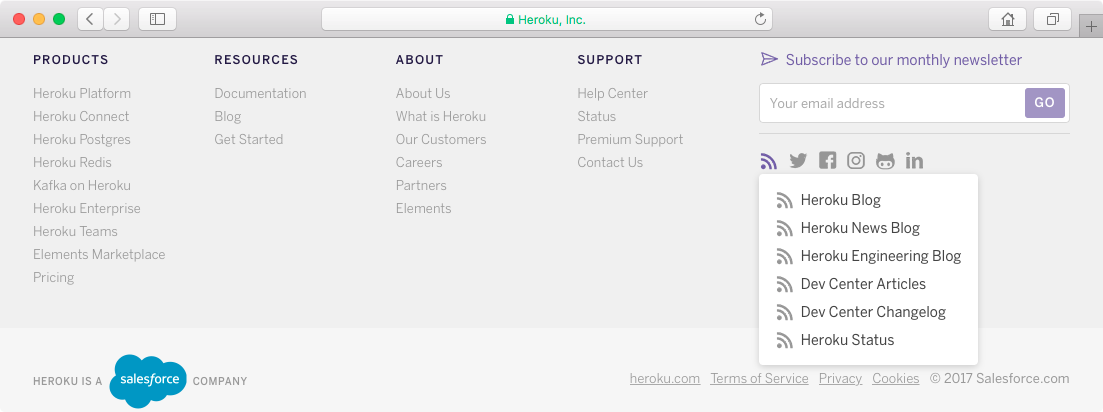
\includegraphics[width=1.0\textwidth]{images/heroku-feeds.png}
	\caption{Feed-Channels von Heroku}
	\label{fig:heroku-feeds}
\end{figure}
Der Themenbereich umfasst sowohl allgemeine (z.B. Heroku Blog) als auch spezifische Informationen (z.B. Dev Center Articles). Im Anwendungsfall von \textit{PaaSfinder} ist der Dev Center Changelog Channel besonders relevant, da der die Benachrichtigungen im technischen Bereich enth�lt (siehe Abbildung \ref{fig:heroku-changelog-feed}).
\begin{figure}[H] 
	\centering
	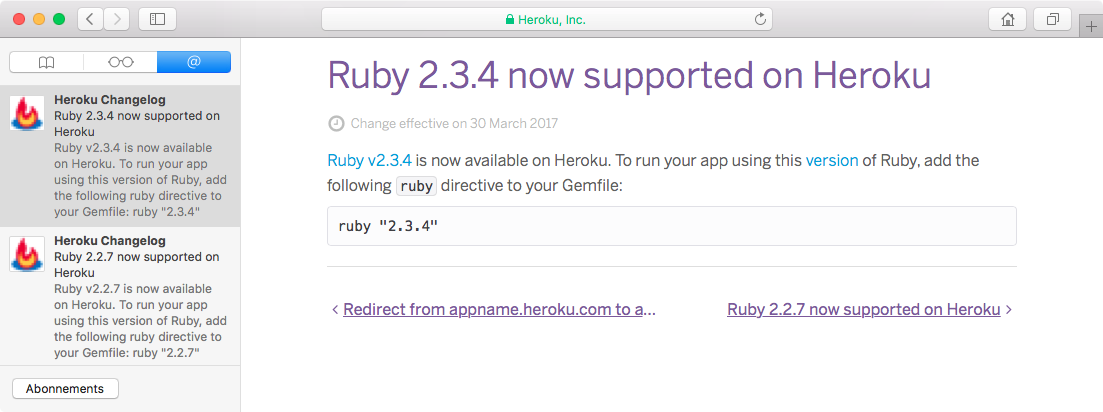
\includegraphics[width=1.0\textwidth]{images/heroku-changelog.png}
	\caption{Heroku Feed}
	\label{fig:heroku-changelog-feed}
\end{figure}
Neben RSS k�nnen die Daten aus sozialen Netzwerken erschlossen werden. Zu diesem Zweck stellen die Anbieter der sozialen Netzwerken (z.B. Facebook\footnote{https://developers.facebook.com/docs/graph-api/}, Twitter\footnote{https://dev.twitter.com/overview/api}) eine REST-API zur Verf�gung, die das Lesen/Schreiben der Daten erm�glicht. Im Beispiel von Heroku hat sich herausgestellt, dass sich Twitter am besten f�r Benachrichtigungen geeignet ist. Bei diesem konkreten Fall handelt es sich sogar um die gleiche Information wie in RSS-Feeds (vgl. Heroku in Abbildung \ref{fig:heroku-changelog-feed} und \ref{fig:heroku-twitter}).
\begin{figure}[H] 
	\centering
	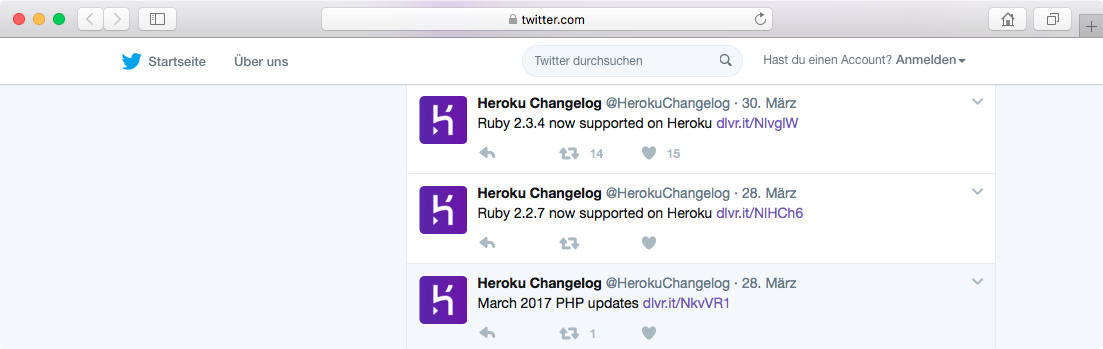
\includegraphics[width=1.0\textwidth]{images/twitter.png}
	\caption{Heroku Twitter}
	\label{fig:heroku-twitter}
\end{figure}
Es bleibt also dem Entwickler offen, ob man sich f�r einen News-Dienst wie Twitter oder Web-Feeds entscheidet. In beiden F�llen kommt man auf die gleiche Information, die unterschiedlich repr�sentiert wird. W�hrend Twitter eine umfangreiche REST-API mit Daten in JSON Format anbietet, setzt RSS auf das XML-Format. Die RSS-Daten k�nnen mit dem HTTP-GET-Request aufgerufen werden.\\
Unabh�ngig davon, ob die Datenerfassung �ber Twitter API oder RSS erfolgt, k�nnen die Daten wiederum an die Worker-API gesendet werden. Im einfachsten Fall werden sie an das Github-Repository weitergegeben. In der fortgeschrittenen Variante k�nnen die Daten nach bestimmten Kriterien gefiltert bzw. verarbeitet werden. 
\subsection{Future Work}\label{subsec:future_work}
Im folgenden Abschnitt werden zuk�nftig m�gliche Arbeitsrichtungen in Bezug auf die Automatisierung der Datenerfassung von \textit{PaaSfinder} erl�utert, die auf den Erkenntnissen aus \ref{subsec:Wissenstr�gerschnittstelle}, \ref{subsec:Worker} und \ref{subsec:vergleich} basieren. \\
Als Weiterentwicklung der Arbeit aus \ref{subsec:Wissenstr�gerschnittstelle} soll Hilfestellung in das Interface eingebaut werden. Da es nicht immer f�r alle Nutzer ersichtlich ist, was ein bestimmtes Feld bedeutet, sollte neben jedem Feld ein Element (z.B. Fragezeichen Tooltip) hinzugef�gt werden, das eine kurze Erkl�rung enth�lt.\\
Zun�chst soll die REST API von Twitter genauer untersucht werden. Da Twitter enorm verbreitet ist, lassen sich Nachrichten vieler Vendors auf einmal erfassen. Die Aufgabe besteht darin, die Daten nach Vendors zu sortieren. Als N�chstes k�nnten die Daten nach einem Muster ausgewertet werden. Wenn beispielsweise das Wort \glqq{}Ruby\grqq{} vorkommt, ist die Wahrscheinlichkeit hoch, dass es sich um ein Update der unterst�tzen Version von Ruby handelt. Hier besteht auch Potential f�r das Anwenden von maschinellem Lernen, indem die Trainingsmengen von Twitter ausgewertet werden. \\
Im Weiteren soll das Potential von Blogs ausgenutzt werden. Die Artikel, die in Blogs pub\-liziert werden, k�nnen zus�tzliche Informationen und externe Links auf wichtige Ressourcen enthalten. Dabei bietet es sich an, einen Web-Crawler zu benutzen. Wenn ein Newsletter allgemein oder im Kontext eines Blogs angeboten wird, kann diese M�glichkeit in Anspruch genommen werden. Ansonsten kann ein Service entwickelt werden, der den Update Reminder an verantwortliche Personen der Firmen via E-Mail nach einem bestimmten Zeitraum nach dem letzten Update verschickt.\\
Schlie�lich sollen die automatischen Tests von \textit{PaaSfinder} erweitert werden, um die Konsistenz der Daten sicherzustellen. Bei der Implementierung der Wissenstr�gerschnittstelle stellte sich als h�ufiges Problem heraus, dass einige Felder auf null gesetzt werden, was zu Problemen bei der Darstellung der Daten f�hrt.
\newpage
\section{Fazit}\label{sec:Fazit}
Im folgenden Abschnitt handelt es sich um die Zusammenfassung der Ergebnisse, die im Zuge dieser Arbeit entstanden sind. Allgemein lassen sich die Ergebnisse aus der theoretischen und der praktischen Sicht betrachten.\\
Im theoretischen Teil wurden zun�chst die Grundlagen von wissensbasierten bzw. Expertensystemen umfassend analysiert. 
Im Weiteren wurde der Schwerpunkt auf die genaue Untersuchung der Wissenserwerbskomponente gelegt. Daraus ist ein Modell der Wissenserwerbs entstanden (siehe Abbildung \ref{fig:wissenserwerbskomponente}), das drei Kategorien des Wissenserwerbs unterscheidet, n�mlich indirekter, direkter und automatisierter Wissenserwerb. Dar�ber hinaus wurde die Komponente zur Daten�bermittlung definiert, die als Bindeglied zwischen den Wissenserwerbsmethoden und der Wissensbasis auftritt.\\
Bez�glich der Wissenserwerbsmethoden wurden zahlreiche Arbeiten untersucht, die sich mit direkten und automatisierten Wissenserwerbsmethoden besch�ftigen. Meistens handelte es sich um den Einsatz vom maschinellen Lernen beim automatisieren Wissenserwerb. In \cite{tecuci1992} und \cite{castro2001} wurde allerdings betont, dass das maschinelle Lernen in Kooperation mit einem fachlichen Experten am besten funktioniert. Ein anderer Ansatz wird in \cite{gebus2009} vorgestellt. In dieser Fallstudie liegt der Fokus auf der Mensch-Computer-Interaktion. Um Erfahrungswissen aus der Produktionsabteilung zu erfassen, verwenden die Autoren eine graphische Benutzerschnittstelle zur Dateneingabe. Ein anderer Bereich, in dem die Datenerfassung eine zunehmende Bedeutung hat, stellt das Web dar. Dieses Interesse ist in der ersten Linie durch die enorm schnelle Entwicklung des Web und damit verbundenen Datenmengen begr�ndet. Einen umfassend �berblick kann man aus der Abrbeit von Ferrara et al \cite{ferrara2014} entnehmen.\\
Im praktischen Teil geht es um die Anwendung der theoretischen Erkenntnisse auf \textit{PaaSfinder}. Als erstes wurde die Idee der Wissenstr�gerschnittstelle umgesetzt, sodass der Nutzer der Wissensbasis von \textit{PaaSfinder} ohne Informatikvorkenntnisse beitragen kann. Die Implementierung umfasst zwei Teile. Im ersten Teil wurde das Frontend entwickelt, das die Daten dynamisch aktualisieren l�sst und im lokalen Speicher f�r sp�tere �bermittlung verwaltet. Im zweiten Teil wurde ein Service implementiert, der f�r die Weiterleitung der Daten an die Wissensbasis (das Git-Repository) zust�ndig ist. Der Service verwendet wiederum die API von Github, um die Daten abzuschicken.\\
Im Weiteren wurden die M�glichkeiten untersucht, die potentiell bei der Automatisierung der Datenerfassung bei \textit{PaaSfinder} benutzt werden k�nnen. Allgemein wurden drei Informationsquellen betrachtet, n�mlich die Webseiten von PaaS-Anbietern, Web-Feeds und soziale Netzwerke. Die Webseiten bieten einen Informationsmehrwert, wenn es sich um einen nicht erfassten PaaS-Anbieter handelt. F�r die Aktualisierungen auf der Webseite sind eher zeitlich geordnete Web-Feeds geeignet. Alternativ k�nnen die Updates aus sozialen Netzwerken (z.B. Facebook, Twitter etc.) bezogen werden.
\newpage

% Einstellungen f�r Literaturverzeichnis
\addcontentsline{toc}{section}{\bibname}
\bibliographystyle{geralpha}
\selectlanguage{german}

% Hier das Literaturverzeichnis einbinden
\bibliography{bibliography/references}
\newpage

% Eigenst�ndigkeitserkl�rung
\makedeclaration{Bachelorarbeit}{16.05.2017}{Petr Vasilyev}

\end{document}